\documentclass{beamer}
\usepackage{xcolor}
% \usetheme{Marburg}
\usecolortheme{orchid}
\usepackage{pifont}
\usepackage{nicefrac}
\usepackage{csquotes}
\usepackage{changepage}
\usepackage{cancel}  
\makeatletter
\def\blfootnote{\gdef\@thefnmark{}\@footnotetext}
\makeatother
\newcommand{\crossout}[2][red]{%
  \begin{tikzpicture}[baseline=(texte.base)]
    % Nœud pour le texte
    \node[inner sep=0pt, outer sep=0pt] (texte) {#2};
    % Dessiner la croix (deux lignes diagonales)
    \draw[overlay, #1, line width=0.5pt] 
      (texte.north west) -- (texte.south east); % Ligne diagonale 1
    \draw[overlay, #1, line width=0.5pt] 
      (texte.north east) -- (texte.south west); % Ligne diagonale 2
  \end{tikzpicture}%
}
\setbeamertemplate{navigation symbols}{}
\usepackage[  
backend=biber,
style=alphabetic,
]{biblatex}
\addbibresource{../../bib/these.bib}
\usepackage{hyperref, xcolor, cmbright,diagbox,colortbl,tikz,graphicx,algorithm2e,cancel,verbatim, graphicx,
listings,float,amsmath,amssymb,array,subfiles,bussproofs,
rotating,MnSymbol,hyperref,mathtools,subcaption,caption}
\newtheorem{proposition}{Proposition}
\usetikzlibrary{overlay-beamer-styles}
\usetikzlibrary{automata, positioning,graphs,shapes, arrows, calc}

\newcommand{\set}[1]{\{#1\}}
\newcommand{\vertex}[2]{%
  \begin{tikzpicture}[baseline=-1ex]%
    \node [rectangle,rounded corners=2mm,inner sep=0.5mm,fill=#2] {$#1$};%
  \end{tikzpicture}%
}
\newcommand{\graphbox}[8]{
  \begin{scope}[xshift=#2,yshift=#3]
    \draw [rounded corners=2mm] (0,0) rectangle (#4,-#5);
    \node at (0,0mm) [anchor=north west,inner sep=1mm] {#1};
    \begin{scope}[xshift=#4/2+#6,yshift=#7] 
    #8
    \end{scope}
  \end{scope}
}

\newcommand{\opn}[1]{\operatorname{#1}}

\graphicspath{ {.} }

\title{Automated Termination Proving: Contributions to Graph Rewriting\\via Extended Weighted Type Graphs\\and Morphism Counting}
\setbeamertemplate{footline}[frame number]


\usetheme{default}% base theme

% default appearance
% \setbeamercolor{structure}{fg=blue}

% % code run at the start of each \section
% \AtBeginSection[]{
%   % a simple section title slide
%   \begin{frame}[plain]
%     \centering\Huge\insertsection
%   \end{frame}

%   % change appearance depending on section number
%   \ifcase\value{section} % 0 (no section) -> fallthrough to default
%   \or % section 1
%     \setbeamercolor{structure}{fg=blue}
%     \usebackgroundtemplate{} % clear background
%     \setcounter{framenumber}{0}%
%   \or % section 2
%     \setbeamercolor{structure}{fg=teal}
%     \usebackgroundtemplate{\includegraphics[width=\paperwidth,height=\paperheight]{bg-section2.pdf}}
%     \setcounter{framenumber}{0}%
%   \or % section 3
%     \setbeamercolor{structure}{fg=violet}
%     \usebackgroundtemplate{\tikz[overlay,remember picture] \fill[black!10] (current page.south west) rectangle (current page.north east);}
%     \setcounter{framenumber}{0}%
%   \else
%     % fallback for later sections
%     \setbeamercolor{structure}{fg=black}
%     \usebackgroundtemplate{}
%   \fi
% }

\begin{document}
% \date{\today}
\date{}
\author{Qi QIU}
\institute[VFU] % (optional)
{
	Supervisor: Xavier URBAIN\\
	Université Claude Bernard Lyon 1, France \\
  Université de Lorraine, France\\
}

\maketitle
% \begin{frame}{Outline}
%   \tableofcontents[hideallsubsections]
% \end{frame} 
\section{Introduction}
\begin{frame}
  \tableofcontents
\end{frame}

\begin{frame}{Rule-based Graph Rewriting and Distributed algorithms}
    \begin{itemize}
        \item Correctness of distributed algorithms is hard to ensure.
        \item Rule-based graph rewriting for modeling distributed algorithms:
             \begin{itemize}
                \item Configurations : graphs
                \item Operations : graph rewriting rules
             \end{itemize}
        \item Automated reasoning for verification
    \end{itemize}
\end{frame}

\subsection{Graphs and Graph Morphisms}
\begin{frame}{Graphs}
\begin{adjustwidth}{-0.5cm}{0cm}
Graphs are \textcolor{red}{finite} and \textcolor{blue}{directed} with:
  \begin{itemize}
      \item Labeled edges,
      \item Finite labels,
      \item Distinct edges with the same source, target, and label
  \end{itemize}
      Example: 
        \begin{center} 
          \resizebox{0.5\textwidth}{!}{
          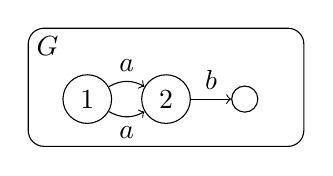
\begin{tikzpicture}
              \graphbox{\(G\)}{00mm}{-20mm}{35mm}{15mm}{2mm}{-5mm}{ 
                  \coordinate (o) at (-2mm,-4mm); 
                  \node[draw,circle] (l1) at ($(o)+(-10mm,0mm)$) {1};
                  \node[draw,circle] (l3) at ($(l1)+(1,0)$) {2};
                  \node[draw,circle] (l4) at ($(l1)+(2,0)$) {};
                  \draw[->] (l1) edge[bend right]  node[midway,below] {$a$} (l3);
                  \draw[->] (l1) edge[bend left] node[midway,above] {$a$}  (l3);
                  \draw[->] (l3) -- (l4) node[midway,above] {$b$};
                  % \draw[->] (l4) -- (l2) node[midway,above] {$a$};
              }   
          \end{tikzpicture} 
      }
      \end{center}
      \begin{itemize}
            \item Enclosed in a box
            \item Graph name $G$ in the top left corner
            \item Numbers in nodes are identifiers, ommitted when not relevant.
      \end{itemize}
\end{adjustwidth}
\end{frame} 

\begin{frame}{Graph Morphisms}
\begin{adjustwidth}{-0.5cm}{0cm}
  \begin{itemize}
      \item \textbf{Graph morphisms} are structure-preserving mappings.
      \item Example of a morphism $h: G \rightarrow H$:
         \begin{center}
          \resizebox{0.8\textwidth}{!}{
          \begin{tikzpicture}
            \graphbox{\( G \)}{0mm}{-20mm}{45mm}{25mm}{2mm}{-10mm}{
                \coordinate (o) at (-5mm,-8mm); 
                \node[draw,circle] (l1) at ($(o)+(-10mm,0mm)$) {1};
                \node[draw,circle] (l2) at ($(l1)+(3,0)$) {2};
                \node[draw,circle] (l3) at ($(l1)+(1,0)$) {3};
                \node[draw,circle] (l4) at ($(l1)+(2,0)$) {4};
                \draw[->] (l1) -- (l3) node[midway,above] {$a$};
                \draw[->] (l3) -- (l4) node[midway,above] {$b$};
                \draw[->] (l4) -- (l2) node[midway,above] {$a$};
            }  
            \graphbox{\( H \)}{52mm}{-20mm}{50mm}{25mm}{2mm}{-10mm}{
                \coordinate (o) at (-5mm,-8mm); 
                \node[draw,circle] (l1) at ($(o)+(-1,0mm)$) {1};
                \node[draw,circle] (l2) at ($(l1)+(3,0)$) {2};
                \node[draw,circle] (l3) at ($(l1)+(1.5,0)$) {3\ 4};
                \draw[->] (l1) edge node[midway,above] {$a$} (l3);
                \draw[->] (l3) edge [loop above] node[midway,above] {$b$} (l3) ;
                \draw[->] (l3) -- (l2) node[midway,above] {$a$};
            }      
            \node () at (48mm,-30mm) {$\overset{h}{\rightarrow}$};
        \end{tikzpicture}
          }
         \end{center}
       \item Isomorphisms: bijective morphisms.
       \item Inclusions : morphisms with $f(x) = x$ for all $x$ from the domain.
       \item Example of an inclusion:
         \begin{center} 
            \resizebox{0.7\textwidth}{!}{
                \begin{tikzpicture}
                    \graphbox{$L$}{39mm}{0mm}{35mm}{35mm}{2mm}{-5mm}{
                        \coordinate (delta) at (0,-18mm);
                        \node[draw,circle,red] (l1) at ($(delta)+(-1,1.5)$) {1};
                        \node[draw,circle,red] (l2) at ($(delta)+(1,1.5)$) {2};
                        \node[draw,circle,red] (l3) at ($(delta)+(0,0)$) {3};
                        \draw[->,red] (l1) -- (l3) node[midway,left] {$s$};
                        \draw[->,red] (l2) -- (l3) node[midway,right] {$s$};
                        \draw[->,red] (l3) edge [loop below] node {0} (l3);
                    }
                        \node () at (77mm,-18mm) {$\overset{h}{\rightarrow}$};
                    \graphbox{$R$}{80mm}{0mm}{50mm}{35mm}{2mm}{-5mm}{
                        \coordinate (delta) at (-10mm,-18mm);
                        \node[draw,circle,red] (r1) at ($(delta)+(-1,1.5)$) {1};
                        \node[draw,circle,red] (r2) at ($(delta)+(0.5,1.5)$) {2};
                        \node[draw,circle,red] (r3) at ($(delta)+(0,0)$) {3};
                        \node[draw,circle] (r4) at ($(delta)+(1,0)$) {};
                        \node[draw,circle] (r5) at ($(r2)+(1.5,0)$) {};
                        \draw[->] (r1) edge[bend right] node[midway,left] {$s$} (r3) ; 
                        \draw[->] (r2) -- (r4) node[midway,right] {$s$};
                        \draw[->] (r4) edge [loop below] node {0} (r4);
                        \draw[->] (r5) edge [loop below] node {0} (r5);
                        \draw[->] (r5) edge [loop right] node {0} (r5);
                        \draw[->] (r5) edge [loop left] node {0} (r5);
                        \draw[->,red] (r1) edge node[midway,left] {$s$} (r3) ;
                        \draw[->,red] (r2) edge node[midway,right] {$s$} (r3) ; 
                        \draw[->,red] (r3) edge [loop below] node {0} (r3); 
                    }
                \end{tikzpicture}
                }
        \end{center}
  \end{itemize} 
\end{adjustwidth}
\end{frame}

\subsection{Graph Rewriting}
\begin{frame}{Commutative Diagram}
  A diagram:
     \begin{center}
        \resizebox{0.3\textwidth}{!}{
            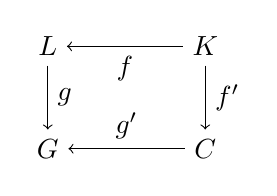
\begin{tikzpicture}
                    \node (I) at (0,-0.7) {$K$};
                    \node (L) at (-2,-0.7) {$L$};
                    \node (G) at (-2,-2) {$G$};
                    \node (C) at (0,-2) {$C$};
                    \draw [->] (I) to  node [midway,below] {$f$} (L);
                    \draw [->] (L) to node [midway,right] {$g$} (G);
                    \draw [->] (I) to node [midway,right] {$f'$} (C);
                    \draw [->] (C) to node [midway,above] {$g'$} (G);
                \end{tikzpicture}
        }
    \end{center}
  is \alert{commutes} if $g \circ f = g' \circ f'$.

  Example:
     \begin{center}
    \resizebox{0.4\textwidth}{!}{
      \begin{tikzpicture}
              \graphbox{\( L\)}{0mm}{0mm}{34mm}{15mm}{2mm}{0mm}{
                  \coordinate (o) at (0mm,-8mm); 
                  \node[draw,circle] (l1) at ($(o)+(-10mm,0mm)$) {1};
                  \node[draw,circle] (l2) at ($(l1)+(2,0)$) {2};
                  \node[orange,draw,circle] (l3) at ($(l1)+(1,0)$) {3};
                  \draw[orange,->] (l1) -- (l3) node[midway,above] {$a$};
                  \draw[orange,->] (l3) -- (l2) node[midway,above] {$a$};
              } 
              \graphbox{\( K \)}{40mm}{0mm}{34mm}{15mm}{2mm}{0mm}{
                  \coordinate (o) at (0mm,-8mm); 
                  \node[draw,circle] (l1) at ($(o)+(-10mm,0mm)$) {1};
                  \node[draw,circle] (l2) at ($(l1)+(2,0)$) {2};
              }  
          
              \graphbox{\( G  \)}{0mm}{-22mm}{34mm}{25mm}{2mm}{-5mm}{
                  \coordinate (o) at (0mm,-3mm); 
                  \node[draw,circle] (l1) at ($(o)+(-10mm,0mm)$) {1};
                  \node[draw,circle] (l2) at ($(l1)+(2,0)$) {2};
                  \node[draw,circle,orange] (l3) at ($(l1)+(1,0)$) {3};
                  \node[blue, draw,circle] (l4) at ($(l2)+(0,-1)$) {6};
                  \draw[orange,->] (l1) -- (l3) node[midway,above] {$a$};
                  \draw[orange,->] (l3) -- (l2) node[midway,above] {$a$};
                  \draw[blue,->] (l2) -- (l4) node[midway,right] {$a$};
              }    
              \graphbox{\( C  \)}{40mm}{-22mm}{34mm}{25mm}{2mm}{-5mm}{
                  \coordinate (o) at (0mm,-3mm); 
                  \node[draw,circle] (l1) at ($(o)+(-10mm,0mm)$) {1};
                  \node[draw,circle] (l2) at ($(l1)+(2,0)$) {2};
                  \node[blue,draw,circle] (l4) at ($(l2)+(0,-1)$) {6};
                  \draw[blue,->] (l2) -- (l4) node[midway,right] {$a$};
              }    
              \node () at (37mm,-8mm) {\( \overset{f}{\leftarrow} \)};  
              \node () at (17mm,-18mm) {\( g\ \downarrow \)};
              \node () at (37mm,-33mm) {\( \overset{g'}{\leftarrow} \)};
              \node () at (52mm,-18mm) {\( f\ \downarrow \)};
      \end{tikzpicture}
      }
   \end{center}
\end{frame}

\begin{frame}{Graph rewriting rule}
  \textcolor{red}{Rules} $\varphi \mathop{=} (L \overset{l}{\leftarrow} K \overset{r}{\rightarrow} R)$ consist of inclusions $l$ and $r$. 
  
  Example:
    \begin{center} 
        \resizebox{0.9\textwidth}{!}{
        $\alpha$ = 
        \begin{tikzpicture}[baseline=-10mm]
            \graphbox{\( L \)}{0mm}{-3mm}{34mm}{12mm}{2mm}{2mm}{
                \coordinate (o) at (0mm,-8mm); 
                \node[draw,circle] (l1) at ($(o)+(-10mm,0mm)$) {1};
                \node[draw,circle] (l2) at ($(l1)+(2,0)$) {2};
                \node[draw,circle] (l3) at ($(l1)+(1,0)$) {3};
                \draw[->] (l1) -- (l3) node[midway,above] {$a$};
                \draw[->] (l3) -- (l2) node[midway,above] {$a$};
            } 

            \graphbox{\( K \)}{40mm}{-3mm}{34mm}{12mm}{2mm}{2mm}{
                \coordinate (o) at (0mm,-8mm); 
                \node[draw,circle] (l1) at ($(o)+(-10mm,0mm)$) {1};
                \node[draw,circle] (l2) at ($(l1)+(2,0)$) {2};
            }  

            \graphbox{\( R \)}{80mm}{-3mm}{45mm}{12mm}{2mm}{2mm}{
                \coordinate (o) at (-5mm,-8mm); 
                \node[draw,circle] (l1) at ($(o)+(-10mm,0mm)$) {1};
                \node[draw,circle] (l2) at ($(l1)+(3,0)$) {2};
                \node[draw,circle] (l3) at ($(l1)+(1,0)$) {4};
                \node[draw,circle] (l4) at ($(l1)+(2,0)$) {5};
                \draw[->] (l1) -- (l3) node[midway,above] {$a$};
                \draw[->] (l3) -- (l4) node[midway,above] {$b$};
                \draw[->] (l4) -- (l2) node[midway,above] {$a$};
            }    
            \node () at (37mm,-8mm) {\( \overset{l}{\leftarrow} \)}; % K -> L
            \node () at (77mm,-8mm) {\( \overset{r}{\rightarrow} \)}; % K -> R
        \end{tikzpicture}
        } 
    \end{center}   

    Rule $\varphi' \mathop{=} (L' \overset{l'}{\leftarrow} K' \overset{r'}{\rightarrow} R')$ and $\varphi$ are \alert{equivalent} if the following commutative diagram can be constructed:
            \begin{center}
                    \resizebox{0.40\textwidth}{!}{
                        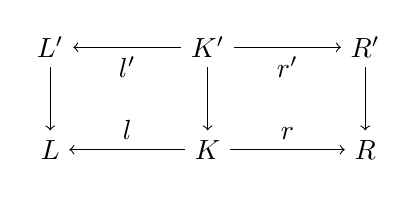
\begin{tikzpicture}
                                \node (I) at (0,-0.7) {$K'$};
                                \node (L) at (-2,-0.7) {$L'$};
                                \node (R) at (2,-0.7) {$R'$};
                                \node (G) at (-2,-2) {$L$};
                                \node (C) at (0,-2) {$K$};
                                \node (H) at (2,-2) {$R$};
                                \draw [->] (I) to  node [midway,below] {$l'$} (L);
                                \draw [->] (I) to  node [midway,below] {$r'$} (R);
                                \draw [->] (L) to node [midway,right] { } (G);
                                \draw [->] (I) to node [midway,right] { } (C);
                                \draw [->] (R) to node [midway,left] { } (H);
                                \draw [->] (C) to node [midway,above] {$l$} (G);
                                \draw [->] (C) to node [midway,above] {$r$} (H);
                                \node [at=($(I)!.5!(G)$)] { };
                                \node [at=($(I)!.5!(H)$)] { };
                            \end{tikzpicture}
                    }
                \end{center}
An equivalent rule of $\alpha$:
    \begin{center}
        \resizebox{0.82\textwidth}{!}{
           \begin{tikzpicture}
                \graphbox{\( L' \)}{0mm}{-3mm}{34mm}{12mm}{2mm}{2mm}{
                    \coordinate (o) at (0mm,-8mm); 
                    \node[draw,circle] (l1) at ($(o)+(-10mm,0mm)$) {6};
                    \node[draw,circle] (l2) at ($(l1)+(2,0)$) {8};
                    \node[draw,circle] (l3) at ($(l1)+(1,0)$) {7};
                    \draw[->] (l1) -- (l3) node[midway,above] {$a$};
                    \draw[->] (l3) -- (l2) node[midway,above] {$a$};
                } 
        
                \graphbox{\( K' \)}{40mm}{-3mm}{34mm}{12mm}{2mm}{2mm}{
                    \coordinate (o) at (0mm,-8mm); 
                    \node[draw,circle] (l1) at ($(o)+(-10mm,0mm)$) {6};
                    \node[draw,circle] (l2) at ($(l1)+(2,0)$) {7};
                }  
        
                \graphbox{\( R' \)}{80mm}{-3mm}{45mm}{12mm}{2mm}{2mm}{
                    \coordinate (o) at (-5mm,-8mm); 
                    \node[draw,circle] (l1) at ($(o)+(-10mm,0mm)$) {6};
                    \node[draw,circle] (l2) at ($(l1)+(3,0)$) {7};
                    \node[draw,circle] (l3) at ($(l1)+(1,0)$) {9};
                    \node[draw,circle] (l4) at ($(l1)+(2,0)$) {10};
                    \draw[->] (l1) -- (l3) node[midway,above] {$a$};
                    \draw[->] (l3) -- (l4) node[midway,above] {$b$};
                    \draw[->] (l4) -- (l2) node[midway,above] {$a$};
                }    
                \node () at (37mm,-8mm) {\( \overset{l'}{\leftarrow} \)};  
                \node () at (77mm,-8mm) {\( \overset{r'}{\rightarrow} \)}; %
            \end{tikzpicture}
            }     
    \end{center}    
\end{frame}

\begin{frame}{Graph Rewriting}
 
 Rewriting steps $G \mathop{\Rightarrow}_\varphi H$ using rule $\varphi$ are commutative diagrams with an equivalent rule $L' \overset{l'}{\leftarrow} K' \overset{r'}{\rightarrow} R'$ where all morphisms are inclusions:
         \begin{center}
          \resizebox{0.40\textwidth}{!}{
              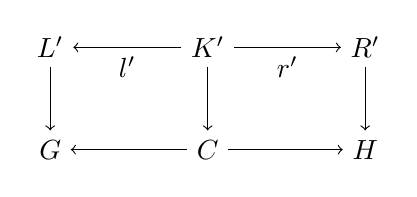
\begin{tikzpicture}
                    \node (I) at (0,-0.7) {$K'$};
                    \node (L) at (-2,-0.7) {$L'$};
                    \node (R) at (2,-0.7) {$R'$};
                    \node (G) at (-2,-2) {$G$};
                    \node (C) at (0,-2) {$C$};
                    \node (H) at (2,-2) {$H$};
                    \draw [->] (I) to  node [midway,below] {$l'$} (L);
                    \draw [->] (I) to  node [midway,below] {$r'$} (R);
                    \draw [->] (L) to node [midway,left] {} (G);
                    \draw [->] (I) to node [midway,right] { } (C);
                    \draw [->] (R) to node [midway,left] { } (H);
                    \draw [->] (C) to node [midway,above] { } (G);
                    \draw [->] (C) to node [midway,above] { } (H);
                    \node [at=($(I)!.5!(G)$)] {} ;
                    \node [at=($(I)!.5!(H)$)] {};
                  \end{tikzpicture}
          }
      \end{center}

%       A rewriting step using $\varphi$:
%   \begin{center}
%     \resizebox{0.7\textwidth}{!}{
%       \begin{tikzpicture}
%               \graphbox{\( L\)}{0mm}{5mm}{34mm}{20mm}{2mm}{-5mm}{
%                   \coordinate (o) at (0mm,-8mm); 
%                   \node[draw,circle] (l1) at ($(o)+(-10mm,0mm)$) {1};
%                   \node[draw,circle] (l2) at ($(l1)+(2,0)$) {2};
%                   \node[orange,draw,circle] (l3) at ($(l1)+(1,0)$) {3};
%                   \draw[orange,->] (l1) -- (l3) node[midway,above] {$a$};
%                   \draw[orange,->] (l3) -- (l2) node[midway,above] {$a$};
%               } 

%               \graphbox{\( K \)}{40mm}{5mm}{34mm}{20mm}{2mm}{-5mm}{
%                   \coordinate (o) at (0mm,-8mm); 
%                   \node[draw,circle] (l1) at ($(o)+(-10mm,0mm)$) {1};
%                   \node[draw,circle] (l2) at ($(l1)+(2,0)$) {2};
%               }  

%               \graphbox{\( R \)}{80mm}{5mm}{45mm}{20mm}{2mm}{-5mm}{
%                   \coordinate (o) at (-5mm,-8mm); 
%                   \node[draw,circle] (l1) at ($(o)+(-10mm,0mm)$) {1};
%                   \node[draw,circle] (l2) at ($(l1)+(3,0)$) {2};
%                   \node[red,draw,circle] (l3) at ($(l1)+(1,0)$) {4};
%                   \node[red,draw,circle] (l4) at ($(l1)+(2,0)$) {5};
%                   \draw[red,->] (l1) -- (l3) node[midway,above] {$a$};
%                   \draw[red,->] (l3) -- (l4) node[midway,above] {$b$};
%                   \draw[red,->] (l4) -- (l2) node[midway,above] {$a$};
%               }    

%               \graphbox{\( G  \)}{0mm}{-22mm}{34mm}{30mm}{2mm}{-10mm}{
%                   \coordinate (o) at (0mm,-3mm); 
%                   \node[draw,circle] (l1) at ($(o)+(-10mm,0mm)$) {1};
%                   \node[draw,circle] (l2) at ($(l1)+(2,0)$) {2};
%                   \node[draw,circle,orange] (l3) at ($(l1)+(1,0)$) {3};
%                   \node[blue, draw,circle] (l4) at ($(l2)+(0,-1)$) {6};
%                   \draw[orange,->] (l1) -- (l3) node[midway,above] {$a$};
%                   \draw[orange,->] (l3) -- (l2) node[midway,above] {$a$};
%                   \draw[blue,->] (l2) -- (l4) node[midway,right] {$a$};
%                 %   \node[blue,draw,circle] (l6) at ($(l1)+(0,-1)$) {7};
%                 %   \draw[blue,<-] (l1) -- (l6) node[midway,left] {$a$};
%               }    

%               \graphbox{\( C  \)}{40mm}{-22mm}{34mm}{30mm}{2mm}{-10mm}{
%                   \coordinate (o) at (0mm,-3mm); 
%                   \node[draw,circle] (l1) at ($(o)+(-10mm,0mm)$) {1};
%                   \node[draw,circle] (l2) at ($(l1)+(2,0)$) {2};
%                   \node[blue,draw,circle] (l4) at ($(l2)+(0,-1)$) {6};
%                   \draw[blue,->] (l2) -- (l4) node[midway,right] {$a$};
%                 %   \node[blue,draw,circle] (l6) at ($(l1)+(0,-1)$) {7};
%                 %   \draw[blue,<-] (l1) -- (l6) node[midway,left] {$a$};
%               }    

%               \graphbox{\( H   \)}{80mm}{-22mm}{45mm}{30mm}{2mm}{-10mm}{
%                   \coordinate (o) at (-5mm,-3mm); 
%                   \node[draw,circle] (l1) at ($(o)+(-10mm,0mm)$) {1};
%                   \node[draw,circle] (l2) at ($(l1)+(3,0)$) {2};
%                   \node[draw,circle,red] (l3) at ($(l1)+(1,0)$) {4};
%                   \node[draw,circle,red] (l4) at ($(l1)+(2,0)$) {5};
%                   \node[blue,draw,circle] (l5) at ($(l2)+(0,-1)$) {6};
%                 %   \node[blue,draw,circle] (l6) at ($(l1)+(0,-1)$) {7};
%                 %   \draw[blue,<-] (l1) -- (l6) node[midway,left] {$a$};
%                   \draw[red,->] (l1) -- (l3) node[midway,above] {$a$};
%                   \draw[red,->] (l3) -- (l4) node[midway,above] {$b$};
%                   \draw[red,->] (l4) -- (l2) node[midway,above] {$a$};
%                   \draw[blue,->] (l2) -- (l5) node[midway,right] {$a$};
%               }    

%               \node () at (37mm,-8mm) {\( \overset{l}{\leftarrow} \)}; % K -> L
%               \node () at (77mm,-8mm) {\( \overset{r}{\rightarrow} \)}; % K -> R
%               \node () at (17mm,-18mm) {\( \downarrow \)};
%               \node () at (37mm,-33mm) {\( \leftarrow \)};
%               \node () at (52mm,-18mm) {\( \downarrow \)};
%               \node () at (92mm,-18mm) {\( \downarrow \)};
%               \node () at (77mm,-33mm) {\( \rightarrow \)}; % C -> H
%       \end{tikzpicture}
%       }
%    \end{center}
\end{frame} 
 
\begin{frame}{A rewriting step with a running example}
  Rewriting rule:
  \begin{center}
    $\varphi$=\resizebox{0.78\textwidth}{!}{
      \begin{tikzpicture}[baseline=-10mm]
              \graphbox{\( L\)}{0mm}{5mm}{34mm}{15mm}{2mm}{0mm}{
                  \coordinate (o) at (0mm,-8mm); 
                  \node[draw,circle] (l1) at ($(o)+(-10mm,0mm)$) {6};
                  \node[draw,circle] (l2) at ($(l1)+(2,0)$) {7};
                  \node[orange,draw,circle] (l3) at ($(l1)+(1,0)$) {8};
                  \draw[orange,->] (l1) -- (l3) node[midway,above] {$a$};
                  \draw[orange,->] (l3) -- (l2) node[midway,above] {$a$};
              } 

              \graphbox{\( K \)}{40mm}{5mm}{34mm}{15mm}{2mm}{0mm}{
                  \coordinate (o) at (0mm,-8mm); 
                  \node[draw,circle] (l1) at ($(o)+(-10mm,0mm)$) {6};
                  \node[draw,circle] (l2) at ($(l1)+(2,0)$) {7};
              }  

              \graphbox{\( R \)}{80mm}{5mm}{45mm}{15mm}{2mm}{0mm}{
                  \coordinate (o) at (-5mm,-8mm); 
                  \node[draw,circle] (l1) at ($(o)+(-10mm,0mm)$) {6};
                  \node[draw,circle] (l2) at ($(l1)+(3,0)$) {7};
                  \node[red,draw,circle] (l3) at ($(l1)+(1,0)$) {9};
                  \node[red,draw,circle] (l4) at ($(l1)+(2,0)$) {10};
                  \draw[red,->] (l1) -- (l3) node[midway,above] {$a$};
                  \draw[red,->] (l3) -- (l4) node[midway,above] {$b$};
                  \draw[red,->] (l4) -- (l2) node[midway,above] {$a$};
              }    
              \node () at (37mm,-3mm) {\( \overset{l}{\leftarrow} \)}; % K -> L
              \node () at (77mm,-3mm) {\( \overset{r}{\rightarrow} \)}; % K -> R
      \end{tikzpicture}
      }
   \end{center}

   An equivalent rewriting rule:
  \begin{center}
    $\varphi'$=\resizebox{0.78\textwidth}{!}{
      \begin{tikzpicture}[baseline=-10mm]
              \graphbox{\( L' \)}{0mm}{5mm}{34mm}{15mm}{2mm}{0mm}{
                  \coordinate (o) at (0mm,-8mm); 
                  \node[draw,circle] (l1) at ($(o)+(-10mm,0mm)$) {1};
                  \node[draw,circle] (l2) at ($(l1)+(2,0)$) {2};
                  \node[orange,draw,circle] (l3) at ($(l1)+(1,0)$) {3};
                  \draw[orange,->] (l1) -- (l3) node[midway,above] {$a$};
                  \draw[orange,->] (l3) -- (l2) node[midway,above] {$a$};
              } 

              \graphbox{\( K' \)}{40mm}{5mm}{34mm}{15mm}{2mm}{0mm}{
                  \coordinate (o) at (0mm,-8mm); 
                  \node[draw,circle] (l1) at ($(o)+(-10mm,0mm)$) {1};
                  \node[draw,circle] (l2) at ($(l1)+(2,0)$) {2};
              }  

              \graphbox{\( R' \)}{80mm}{5mm}{45mm}{15mm}{2mm}{0mm}{
                  \coordinate (o) at (-5mm,-8mm); 
                  \node[draw,circle] (l1) at ($(o)+(-10mm,0mm)$) {1};
                  \node[draw,circle] (l2) at ($(l1)+(3,0)$) {2};
                  \node[red,draw,circle] (l3) at ($(l1)+(1,0)$) {4};
                  \node[red,draw,circle] (l4) at ($(l1)+(2,0)$) {5};
                  \draw[red,->] (l1) -- (l3) node[midway,above] {$a$};
                  \draw[red,->] (l3) -- (l4) node[midway,above] {$b$};
                  \draw[red,->] (l4) -- (l2) node[midway,above] {$a$};
              }    
              \node () at (37mm,-3mm) {\( \overset{l'}{\leftarrow} \)}; 
              \node () at (77mm,-3mm) {\( \overset{r'}{\rightarrow} \)}; 
      \end{tikzpicture}
      }
   \end{center}
  
   A rewriting step $G \Rightarrow_\varphi H$:
  \begin{center}
    \resizebox{0.78\textwidth}{!}{
      \begin{tikzpicture}
              \graphbox{\( L' \)}{0mm}{5mm}{34mm}{15mm}{2mm}{0mm}{
                  \coordinate (o) at (0mm,-8mm); 
                  \node[draw,circle] (l1) at ($(o)+(-10mm,0mm)$) {1};
                  \node[draw,circle] (l2) at ($(l1)+(2,0)$) {2};
                  \node[orange,draw,circle] (l3) at ($(l1)+(1,0)$) {3};
                  \draw[orange,->] (l1) -- (l3) node[midway,above] {$a$};
                  \draw[orange,->] (l3) -- (l2) node[midway,above] {$a$};
              } 

              \graphbox{\( K' \)}{40mm}{5mm}{34mm}{15mm}{2mm}{0mm}{
                  \coordinate (o) at (0mm,-8mm); 
                  \node[draw,circle] (l1) at ($(o)+(-10mm,0mm)$) {1};
                  \node[draw,circle] (l2) at ($(l1)+(2,0)$) {2};
              }  

              \graphbox{\( R' \)}{80mm}{5mm}{45mm}{15mm}{2mm}{0mm}{
                  \coordinate (o) at (-5mm,-8mm); 
                  \node[draw,circle] (l1) at ($(o)+(-10mm,0mm)$) {1};
                  \node[draw,circle] (l2) at ($(l1)+(3,0)$) {2};
                  \node[red,draw,circle] (l3) at ($(l1)+(1,0)$) {4};
                  \node[red,draw,circle] (l4) at ($(l1)+(2,0)$) {5};
                  \draw[red,->] (l1) -- (l3) node[midway,above] {$a$};
                  \draw[red,->] (l3) -- (l4) node[midway,above] {$b$};
                  \draw[red,->] (l4) -- (l2) node[midway,above] {$a$};
              }    
                \graphbox{\( G  \)}{0mm}{-17mm}{34mm}{25mm}{2mm}{-5mm}{
                  \coordinate (o) at (0mm,-3mm); 
                  \node[draw,circle] (l1) at ($(o)+(-10mm,0mm)$) {1};
                  \node[draw,circle] (l2) at ($(l1)+(2,0)$) {2};
                  \node[draw,circle,orange] (l3) at ($(l1)+(1,0)$) {3};
                  \node[blue, draw,circle] (l4) at ($(l2)+(0,-1)$) {6};
                  \draw[orange,->] (l1) -- (l3) node[midway,above] {$a$};
                  \draw[orange,->] (l3) -- (l2) node[midway,above] {$a$};
                  \draw[blue,->] (l2) -- (l4) node[midway,right] {$a$};
              }    
              \graphbox{\( C  \)}{40mm}{-17mm}{34mm}{25mm}{2mm}{-5mm}{
                  \coordinate (o) at (0mm,-3mm); 
                  \node[draw,circle] (l1) at ($(o)+(-10mm,0mm)$) {1};
                  \node[draw,circle] (l2) at ($(l1)+(2,0)$) {2};
                  \node[blue,draw,circle] (l4) at ($(l2)+(0,-1)$) {6};
                  \draw[blue,->] (l2) -- (l4) node[midway,right] {$a$};
              }    
              \graphbox{\( H   \)}{80mm}{-17mm}{45mm}{25mm}{2mm}{-5mm}{
                  \coordinate (o) at (-5mm,-3mm); 
                  \node[draw,circle] (l1) at ($(o)+(-10mm,0mm)$) {1};
                  \node[draw,circle] (l2) at ($(l1)+(3,0)$) {2};
                  \node[draw,circle,red] (l3) at ($(l1)+(1,0)$) {4};
                  \node[draw,circle,red] (l4) at ($(l1)+(2,0)$) {5};
                  \node[blue,draw,circle] (l5) at ($(l2)+(0,-1)$) {6};
                  \draw[red,->] (l1) -- (l3) node[midway,above] {$a$};
                  \draw[red,->] (l3) -- (l4) node[midway,above] {$b$};
                  \draw[red,->] (l4) -- (l2) node[midway,above] {$a$};
                  \draw[blue,->] (l2) -- (l5) node[midway,right] {$a$};
              }    
              \node () at (37mm,-3mm) {\( \overset{l'}{\leftarrow} \)}; 
              \node () at (77mm,-3mm) {\( \overset{r'}{\rightarrow} \)}; 
              \node () at (17mm,-13mm) {\( \downarrow \)};
              \node () at (37mm,-28mm) {\( \leftarrow \)};
              \node () at (52mm,-13mm) {\( \downarrow \)};
              \node () at (92mm,-13mm) {\( \downarrow \)};
              \node () at (77mm,-28mm) {\( \rightarrow \)};  
      \end{tikzpicture}
      }
   \end{center}
    It replaces chain  \tikz[baseline=-0.5ex]{ 
            \node (x) at (0,0) {$\bullet$};  
            \node (y) at (1,0) {$\bullet$};
            \node (z) at (2,0) {$\bullet$};
            \draw[->] (x) -- node[midway,above] {$a$} (y) ;
            \draw[->] (y) -- node[midway,above] {$a$} (z) ;
            } with \tikz[baseline=-0.5ex]{ 
            \node (x) at (0,0) {$\bullet$};  
            \node (y) at (1,0) {$\bullet$};
            \node (z) at (2,0) {$\bullet$};
            \node (w) at (3,0) {$\bullet$};
            \draw[->] (x) -- node[midway,above] {$a$} (y) ;
            \draw[->] (y) -- node[midway,above] {$b$} (z) ;
            \draw[->] (z) -- node[midway,above] {$a$} (w) ;
            }.
\end{frame}


\subsection{Termination of graph rewriting systems}
\begin{frame}{Termination of graph rewriting systems}
  \begin{itemize}
    \item $\mathcal{R}$ : a set of rules
    \item No graph \(G_0\) can be rewritten forever:
         $$G_0 \mathop{\Rightarrow}_\mathcal{R} G_1 \mathop{\Rightarrow}_\mathcal{R} G_2 \mathop{\Rightarrow}_\mathcal{R} \cdots$$
         when using the non-deterministic strategy 
          \begin{center}
              \textcolor{blue}{\enquote{apply rules as long as possible}}
          \end{center}
    \item Aligns with the standard notion of program termination: 
         \begin{center}
            \textcolor{blue}{\enquote{every execution (on any input) eventually halts.}}
          \end{center}
    \item Undecidable in general 
  \end{itemize}
\end{frame}

\begin{frame}{One-rule examples of non-termination and termination}
  \begin{center}  
     Rule $\alpha$ :\resizebox{0.85\textwidth}{!}{
                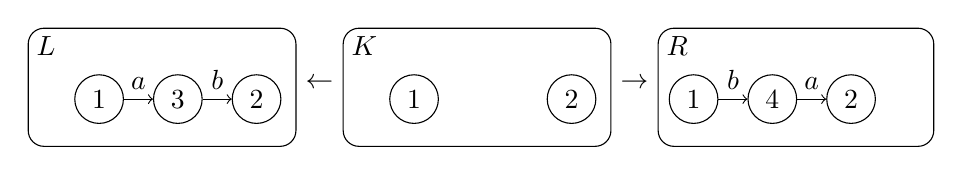
\begin{tikzpicture}[baseline=-10mm]
                    \graphbox{\( L \)}{0mm}{-3mm}{34mm}{15mm}{2mm}{2mm}{
                        \coordinate (o) at (0mm,-11mm); 
                        \node[draw,circle] (l1) at ($(o)+(-10mm,0mm)$) {1};
                        \node[draw,circle] (l2) at ($(l1)+(2,0)$) {2};
                        \node[draw,circle] (l3) at ($(l1)+(1,0)$) {3};
                        \draw[->] (l1) -- (l3) node[midway,above] {$a$};
                        \draw[->] (l3) -- (l2) node[midway,above] {$b$};
                    } 
            
                    \graphbox{\( K \)}{40mm}{-3mm}{34mm}{15mm}{2mm}{2mm}{
                        \coordinate (o) at (0mm,-11mm); 
                        \node[draw,circle] (l1) at ($(o)+(-10mm,0mm)$) {1};
                        \node[draw,circle] (l2) at ($(l1)+(2,0)$) {2};
                    }  
            
                    \graphbox{\( R \)}{80mm}{-3mm}{35mm}{15mm}{2mm}{2mm}{
                        \coordinate (o) at (-5mm,-11mm); 
                        \node[draw,circle] (l1) at ($(o)+(-10mm,0mm)$) {1};
                        % \node[draw,circle] (l2) at ($(l1)+(3,0)$) {2};
                        \node[draw,circle] (l3) at ($(l1)+(1,0)$) {4};
                        \node[draw,circle] (l4) at ($(l1)+(2,0)$) {2};
                        \draw[->] (l1) -- (l3) node[midway,above] {$b$};
                        \draw[->] (l3) -- (l4) node[midway,above] {$a$};
                        % \draw[->] (l4) -- (l2) node[midway,above] {$a$};
                    }    
                    \node () at (37mm,-10mm) {\( \leftarrow \)}; % K -> L
                    \node () at (77mm,-10mm) {\( \rightarrow \)}; % K -> R
                \end{tikzpicture}
                }
            \end{center}  
 
        \begin{center}
            Looping:\resizebox{0.85\textwidth}{!}{
              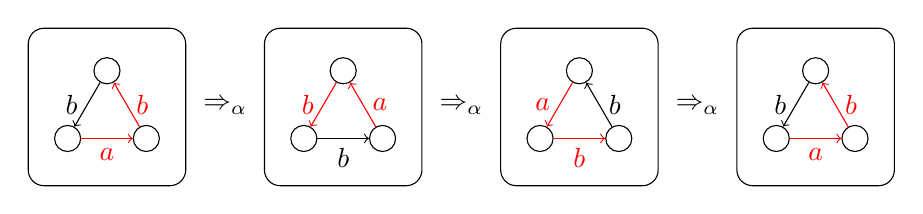
\begin{tikzpicture}[baseline=-10mm]
              \graphbox{\( \)}{0mm}{0mm}{20mm}{20mm}{-5mm}{-14mm}{
                  \node[draw,circle] (x) at (0,0) {};
                  \node[draw,circle] (y) at (1,0) {};
                  \node[draw,circle] (z) at (0.5,0.86) {};
                  \draw[->,red] (x) -- node[midway,below] {$a$} (y) ;
                  \draw[->,red] (y) -- node[midway,right] {$b$} (z) ;
                  \draw[->] (z) -- node[midway,left] {$b$} (x) ;
              } 
              \node () at (25mm,-10mm) {\( \Rightarrow_\alpha \)};
              \graphbox{\( \)}{30mm}{0mm}{20mm}{20mm}{-5mm}{-14mm}{
                  \node[draw,circle] (x) at (0,0) {};  
                  \node[draw,circle] (y) at (1,0) {};
                  \node[draw,circle] (z) at (0.5,0.86) {};
                  \draw[->] (x) -- node[midway,below] {$b$} (y) ;
                  \draw[->,red] (y) -- node[midway,right] {$a$} (z) ;
                  \draw[->,red] (z) -- node[midway,left] {$b$} (x) ;
              } 
              \node () at (55mm,-10mm) {\( \Rightarrow_\alpha \)};
              \graphbox{\( \)}{60mm}{0mm}{20mm}{20mm}{-5mm}{-14mm}{
                  \node[draw,circle] (x) at (0,0) {};  
                  \node[draw,circle] (y) at (1,0) {};
                  \node[draw,circle] (z) at (0.5,0.86) {};
                  \draw[->,red] (x) -- node[midway,below] {$b$} (y) ;
                  \draw[->] (y) -- node[midway,right] {$b$} (z) ;
                  \draw[->,red] (z) -- node[midway,left] {$a$} (x) ;
              }
              \node () at (85mm,-10mm) {\( \Rightarrow_\alpha \)};
              \graphbox{\( \)}{90mm}{0mm}{20mm}{20mm}{-5mm}{-14mm}{
                  \node[draw,circle] (x) at (0,0) {};   
                  \node[draw,circle] (y) at (1,0) {};
                  \node[draw,circle] (z) at (0.5,0.86) {};
                  \draw[->,red] (x) -- node[midway,below] {$a$} (y) ;
                  \draw[->,red] (y) -- node[midway,right] {$b$} (z) ;
                  \draw[->] (z) -- node[midway,left] {$b$} (x) ;
              }
          \end{tikzpicture}
          }
        \end{center}

     
  \begin{center}  
        Rule $b$:\resizebox{0.85\textwidth}{!}{ 
       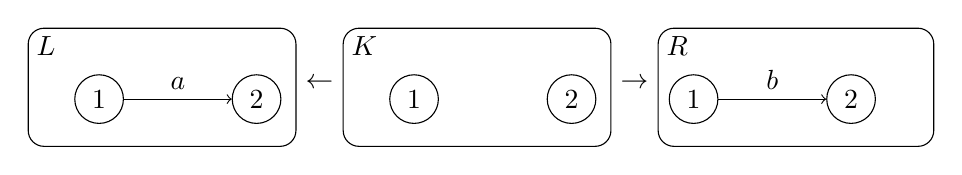
\begin{tikzpicture}[baseline=-10mm]
                    \graphbox{\( L \)}{0mm}{-3mm}{34mm}{15mm}{2mm}{2mm}{
                        \coordinate (o) at (0mm,-11mm); 
                        \node[draw,circle] (l1) at ($(o)+(-10mm,0mm)$) {1};
                        \node[draw,circle] (l2) at ($(l1)+(2,0)$) {2};
                        % \node[draw,circle] (l3) at ($(l1)+(1,0)$) {3};
                        \draw[->] (l1) -- (l2) node[midway,above] {$a$};
                    } 
            
                    \graphbox{\( K \)}{40mm}{-3mm}{34mm}{15mm}{2mm}{2mm}{
                        \coordinate (o) at (0mm,-11mm); 
                        \node[draw,circle] (l1) at ($(o)+(-10mm,0mm)$) {1};
                        \node[draw,circle] (l2) at ($(l1)+(2,0)$) {2};
                    }  
            
                    \graphbox{\( R \)}{80mm}{-3mm}{35mm}{15mm}{2mm}{2mm}{
                        \coordinate (o) at (-5mm,-11mm); 
                        \node[draw,circle] (l1) at ($(o)+(-10mm,0mm)$) {1};
                        % \node[draw,circle] (l2) at ($(l1)+(3,0)$) {2};
                         % \node[draw,circle] (l3) at ($(l1)+(1,0)$) {4};
                        \node[draw,circle] (l4) at ($(l1)+(2,0)$) {2};
                        \draw[->] (l1) -- (l4) node[midway,above] {$b$};
                        % \draw[->] (l4) -- (l2) node[midway,above] {$a$};
                    }    
                    \node () at (37mm,-10mm) {\( \leftarrow \)}; % K -> L
                    \node () at (77mm,-10mm) {\( \rightarrow \)}; % K -> R
                \end{tikzpicture}
                }
            \end{center}  
\vspace{2mm}
\textcolor{blue}{Termination} by the number of edges labeled by \enquote{a}:

        \begin{center}
          \resizebox{0.4\textwidth}{!}{
              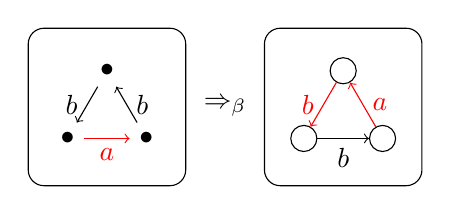
\begin{tikzpicture}
                \graphbox{\( \)}{0mm}{0mm}{20mm}{20mm}{-5mm}{-14mm}{
                  \node (x) at (0,0) {$\bullet$};  
                  \node (y) at (1,0) {$\bullet$};
                  \node (z) at (0.5,0.86) {$\bullet$};
                  \draw[->,red] (x) -- node[midway,below] {$a$} (y) ;
                  \draw[->] (y) -- node[midway,right] {$b$} (z) ;
                  \draw[->] (z) -- node[midway,left] {$b$} (x) ;
                } 
                \node () at (25mm,-10mm) {\( \Rightarrow_\beta \)};
                \graphbox{\( \)}{30mm}{0mm}{20mm}{20mm}{-5mm}{-14mm}{
                    \node[draw,circle] (x) at (0,0) {};  
                    \node[draw,circle] (y) at (1,0) {};
                    \node[draw,circle] (z) at (0.5,0.86) {};
                    \draw[->] (x) -- node[midway,below] {$b$} (y) ;
                    \draw[->,red] (y) -- node[midway,right] {$a$} (z) ;
                    \draw[->,red] (z) -- node[midway,left] {$b$} (x) ;
                }
            \end{tikzpicture}
          }
        \end{center}
\end{frame}

\section{Termination using Morphism Counting}
\begin{frame}
  \tableofcontents[currentsection,hideothersubsections]
\end{frame}

\subsection{Implicit, Explicit and Shared Occurrences}
\begin{frame}{Pre-graphs}
 Pre-graphs are \textbf{graphs with missing nodes} and dangling edges.
 
 Example:

        \begin{center}
            \resizebox{0.6\textwidth}{!}{
            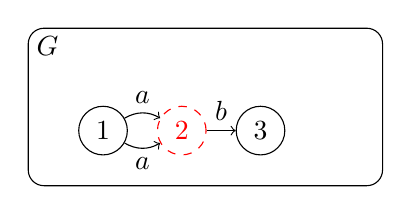
\begin{tikzpicture}
                \graphbox{\( G \)}{00mm}{-20mm}{45mm}{20mm}{2mm}{-5mm}{ 
                    \coordinate (o) at (-5mm,-8mm); 
                    \node[draw,circle] (l1) at ($(o)+(-10mm,0mm)$) {1};
                    % \node[draw,circle] (l2) at ($(l1)+(3,0)$) {};
                    \node[draw,circle,dashed,red] (l3) at ($(l1)+(1,0)$) {2};
                    \node[draw,circle] (l4) at ($(l1)+(2,0)$) {3};
                    \draw[->] (l1) edge[bend right]  node[midway,below] {$a$} (l3);
                    \draw[->] (l1) edge[bend left] node[midway,above] {$a$}  (l3);
                    \draw[->] (l3) -- (l4) node[midway,above] {$b$};
                    % \draw[->] (l4) -- (l2) node[midway,above] {$a$};
                }  
            \end{tikzpicture} 
        }
        \end{center} 

   $G$ has 
    \begin{itemize}
      \item 2 existing nodes,
      \item 1 missing node in red,
      \item 3 dangling edges.
    \end{itemize}
\end{frame}

\begin{frame}{Pre-graph operations}
    \textcolor{red}{Union} of two pre-graphs $C \mathop{\subseteq} G$ and $R \mathop{\subseteq} G$, denoted $C \mathop{\cup} R$:
    % \vspace{1mm}
\begin{center}
    \resizebox{\textwidth}{!}{
        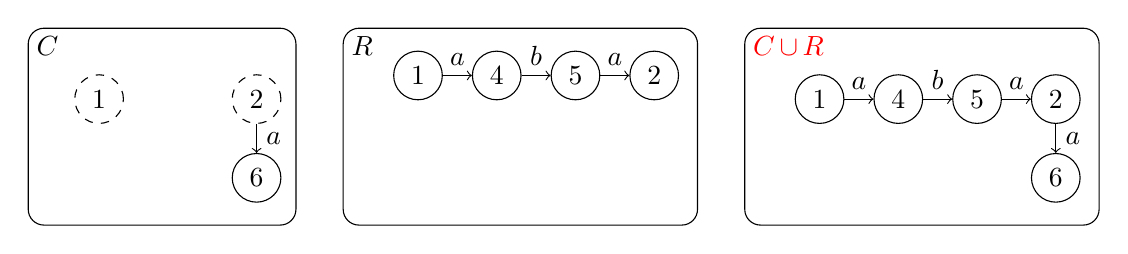
\begin{tikzpicture}          
            \graphbox{\( C  \)}{0mm}{-22mm}{34mm}{25mm}{2mm}{-3mm}{
                \coordinate (o) at (0mm,-6mm); 
                \node[draw,circle,dashed] (l1) at ($(o)+(-10mm,0mm)$) {1};
                \node[draw,circle,dashed] (l2) at ($(l1)+(2,0)$) {2};
                \node[draw,circle] (l4) at ($(l2)+(0,-1)$) {6};
                \draw[->] (l2) -- (l4) node[midway,right] {$a$};
                % \draw[->] (l2) edge[out=-135,in=-45]node[midway,below] {$a$} (l1) ;
                % \node[ draw,circle] (l6) at ($(l1)+(0,-1)$) {7};
                % \draw[<-] (l1) -- (l6) node[midway,left] {$a$};
            }    
            \graphbox{\( R \)}{40mm}{-22mm}{45mm}{25mm}{2mm}{2mm}{
                \coordinate (o) at (-5mm,-8mm); 
                \node[draw,circle] (l1) at ($(o)+(-10mm,0mm)$) {1};
                \node[draw,circle] (l2) at ($(l1)+(3,0)$) {2};
                \node[draw,circle] (l3) at ($(l1)+(1,0)$) {4};
                \node[draw,circle] (l4) at ($(l1)+(2,0)$) {5};
                \draw[->] (l1) -- (l3) node[midway,above] {$a$};
                \draw[->] (l3) -- (l4) node[midway,above] {$b$};
                \draw[->] (l4) -- (l2) node[midway,above] {$a$};
            } 
            \graphbox{\textcolor{red}{\(C \mathop{\cup} R \)}}{91mm}{-22mm}{45mm}{25mm}{2mm}{-3mm}{
                \coordinate (o) at (-5mm,-6mm); 
                \node[draw,circle] (l1) at ($(o)+(-10mm,0mm)$) {1};
                \node[draw,circle] (l2) at ($(l1)+(3,0)$) {2};
                \node[draw,circle] (l3) at ($(l1)+(1,0)$) {4};
                \node[draw,circle] (l4) at ($(l1)+(2,0)$) {5};
                \node[ draw,circle] (l5) at ($(l2)+(0,-1)$) {6};
                % \node[ draw,circle] (l6) at ($(l1)+(0,-1)$) {7};
                % \draw[<-] (l1) -- (l6) node[midway,left] {$a$};
                \draw[->] (l1) -- (l3) node[midway,above] {$a$};
                \draw[->] (l3) -- (l4) node[midway,above] {$b$};
                \draw[->] (l4) -- (l2) node[midway,above] {$a$};
                \draw[->] (l2) -- (l5) node[midway,right] {$a$};
                % \draw[->] (l2) edge[out=-135,in=-45]node[midway,below] {$a$} (l1) ;
            }    
             
        \end{tikzpicture}
    }
    \end{center}
\textcolor{red}{Relative complement} of $R$ in $H$ where $R \mathop{\subseteq} H$, denoted $H \mathop{\setminus} R$: 
    \begin{center}
  \resizebox{\textwidth}{!}{
        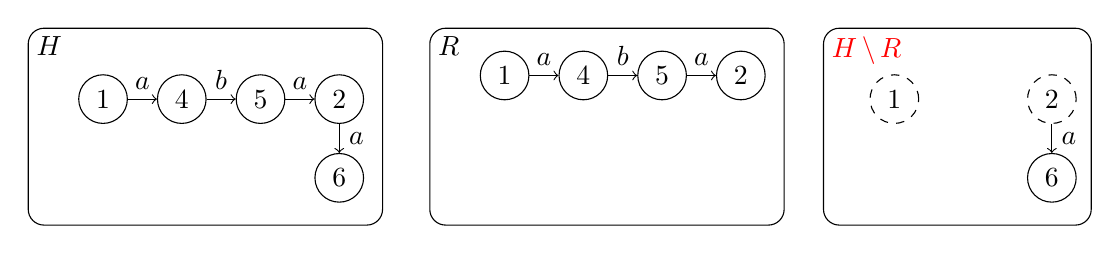
\begin{tikzpicture}       
            \graphbox{\( H \)}{-11mm}{-22mm}{45mm}{25mm}{2mm}{-3mm}{
                \coordinate (o) at (-5mm,-6mm); 
                \node[draw,circle] (l1) at ($(o)+(-10mm,0mm)$) {1};
                \node[draw,circle] (l2) at ($(l1)+(3,0)$) {2};
                \node[draw,circle] (l3) at ($(l1)+(1,0)$) {4};
                \node[draw,circle] (l4) at ($(l1)+(2,0)$) {5};
                \node[ draw,circle] (l5) at ($(l2)+(0,-1)$) {6};
                \draw[->] (l1) -- (l3) node[midway,above] {$a$};
                \draw[->] (l3) -- (l4) node[midway,above] {$b$};
                \draw[->] (l4) -- (l2) node[midway,above] {$a$};
                \draw[->] (l2) -- (l5) node[midway,right] {$a$};
                % \draw[->] (l2) edge[out=-135,in=-45]node[midway,below] {$a$} (l1) ;
            }  
            \graphbox{\( R \)}{40mm}{-22mm}{45mm}{25mm}{2mm}{2mm}{
                \coordinate (o) at (-5mm,-8mm); 
                \node[draw,circle] (l1) at ($(o)+(-10mm,0mm)$) {1};
                \node[draw,circle] (l2) at ($(l1)+(3,0)$) {2};
                \node[draw,circle] (l3) at ($(l1)+(1,0)$) {4};
                \node[draw,circle] (l4) at ($(l1)+(2,0)$) {5};
                \draw[->] (l1) -- (l3) node[midway,above] {$a$};
                \draw[->] (l3) -- (l4) node[midway,above] {$b$};
                \draw[->] (l4) -- (l2) node[midway,above] {$a$};
            }     
            \graphbox{\textcolor{red}{\( H \mathop{\setminus} R  \)}}{90mm}{-22mm}{34mm}{25mm}{2mm}{-3mm}{
                \coordinate (o) at (0mm,-6mm); 
                \node[draw,dashed,circle] (l1) at ($(o)+(-10mm,0mm)$) {1};
                \node[draw,dashed,circle] (l2) at ($(l1)+(2,0)$) {2};
                \node[draw,circle] (l4) at ($(l2)+(0,-1)$) {6};
                \draw[->] (l2) -- (l4) node[midway,right] {$a$};
                % \draw[->] (l2) edge[out=-135,in=-45]node[midway,below] {$a$} (l1) ;
            }   
        \end{tikzpicture}
    }
    \end{center}

    % Remark : \textcolor{red}{$H \mathop{\setminus} R$ is not always a graph.}
\end{frame}



\begin{frame}{Analysis of rewriting steps} 
       
    In a rewriting step, since all arrows are inclusions by definition,
    graphs can be decomposed as unions of pre-graphs:
   \begin{center}
       \resizebox{0.4\textwidth}{!}{
        \begin{tikzpicture}
            % [node distance=15mm]
            \node (I) at (0,0) {$K$};
            \node (L)  at (-3,0) {$L' \cup K$};
            \node (R)  at (3,0) {$R' \cup K$};
            \node (G)  at (-3,-3) {$L' \cup K \cup C'$};
            \node (C)  at (0,-3) {$K \cup C'$};
            \node (H)  at (3,-3) {$R' \cup K \cup C'$};
            \draw [->] (I) to  node [midway,below] {} (L);
            \draw [->] (I) to  node [midway,below] {} (R);
            \draw [->] (L) to node [midway,right] {} (G);
            \draw [->] (I) to  node [midway,right] {} (C);
            \draw [->] (R) to  node [midway,right] {} (H);
            \draw [->] (C) to node [midway,above] {} (G);
            \draw [->] (C) to node [midway,above] {} (H);
        \end{tikzpicture}
    }
    \hspace{0.8cm}
    \resizebox{0.4\textwidth}{!}{
            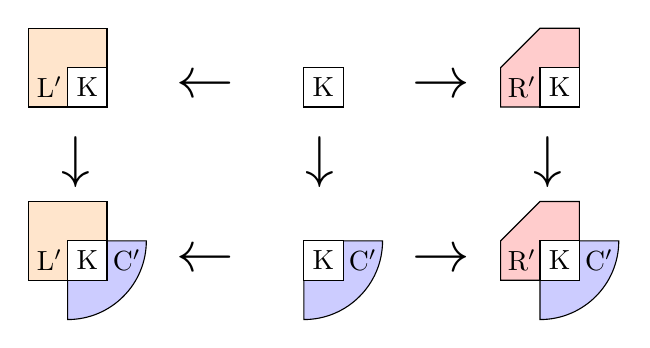
\begin{tikzpicture} 
                \coordinate (k) at (0, 0);
                \draw[fill=white] ($(k)+(0,0)$) rectangle ($(k)+(0.5,0.5)$);
                \node () at ($(k)+(0.25,0.25)$) {\( \mathrm{K} \)};
            
                \coordinate (c) at (0, -2.2);
                \draw[fill=blue!20]
                ($(c)+(0,-0.5)$)
                -- ($(c)+(0,0.5)$) 
                -- ($(c)+(1,0.5)$) 
                arc[start angle=0, end angle=-90, radius=1]
                -- cycle;
                \node () at ($(c)+(0.75,0.25)$) {\( \mathrm{C'} \)};
                \draw[fill=white] ($(c)+(0,0)$) rectangle ($(c)+(0.5,0.5)$);
                \node () at ($(c)+(0.25,0.25)$) {\( \mathrm{K} \)};
            
                \coordinate (l) at (-3, 0);
                \draw[fill=orange!20] ($(l)+(-0.5,0)$) rectangle ($(l)+(0.5,1)$);
                \node () at ($(l)+(-0.23,0.25)$) {\( \mathrm{L'} \)};
                \draw[fill=white] ($(l)+(0,0)$) rectangle ($(l)+(0.5,0.5)$);
                \node () at ($(l)+(0.25,0.25)$) {\( \mathrm{K} \)};
            
                \coordinate (g) at (-3, -2.2);
                \draw[fill=blue!20]
                ($(g)+(0,-0.5)$)
                -- ($(g)+(0,0.5)$)
                -- ($(g)+(1,0.5)$) 
                arc[start angle=0, end angle=-90, radius=1]
                -- cycle;
                \draw[fill=orange!20] ($(g)+(-0.5,0)$) rectangle ($(g)+(0.5,1)$);
                \node () at ($(g)+(0.75,0.25)$) {\( \mathrm{C'} \)};
                \node () at ($(g)+(-0.23,0.25)$) {\( \mathrm{L'} \)};
                \draw[fill=white] ($(g)+(0,0)$) rectangle ($(g)+(0.5,0.5)$);
                \node () at ($(g)+(0.25,0.25)$) {\( \mathrm{K} \)};
            
                \coordinate (r) at (3,0);
                \draw[fill=red!20] ($(r)+(-0.5,0)$)
                -- ($(r)+(-0.5,0.5)$)
                -- ($(r)+(0,1)$)
                --  ($(r)+(0.5,1)$)
                -- ($(r)+(0.5,0)$)
                -- cycle;
                \node () at ($(r)+(-0.23,0.25)$) {\( \mathrm{R'} \)};
                \draw[fill=white] ($(r)+(0,0)$) rectangle ($(r)+(0.5,0.5)$);
                \node () at ($(r)+(0.25,0.25)$) {\( \mathrm{K} \)};
            
                \coordinate (h) at (3, -2.2);
                \draw[fill=blue!20]
                ($(h)+(0,-0.5)$)
                -- ($(h)+(0,0.5)$)
                -- ($(h)+(1,0.5)$) 
                arc[start angle=0, end angle=-90, radius=1]
                -- cycle;
                \draw[fill=red!20] ($(h)+(-0.5,0)$)
                -- ($(h)+(-0.5,0.5)$)
                -- ($(h)+(0,1)$)
                --  ($(h)+(0.5,1)$)
                -- ($(h)+(0.5,0)$)
                -- cycle;
            \node () at ($(h)+(0.75,0.25)$) {\( \mathrm{C'} \)};
            \draw[fill=white] ($(h)+(0,0)$) rectangle ($(h)+(0.5,0.5)$);
            \node () at ($(h)+(0.25,0.25)$) {\( \mathrm{K} \)};
            \node () at ($(h)+(-0.23,0.25)$) {\( \mathrm{R'} \)};
            
                \node[ font=\huge] (kl) at ($(k)!0.5!(l)+(0.25,0.25)$)
            %    {\( \overset{l}{\leftarrow} \)}
                {\( \leftarrow \)}
                ; 
                \node[ font=\huge] (kr) at ($(k)!0.5!(r)+(0.25,0.25)$)
                {\( \rightarrow \)}
                ;  
                \node[ font=\huge] (cg) at ($(c)!0.5!(g)+(0.25,0.25)$) 
                {\( \leftarrow \)}
            ;  
                \node[ font=\huge] (ch) at ($(c)!0.5!(h)+(0.25,0.25)$)
                {\( \rightarrow \)}
            ; 
                \node[ font=\huge] (kc) at ($(k)!0.5!(c)+(0.2,0.4)$) {\( \downarrow \)}; 
            %   \node[ font=\LARGE] () at ($(l)!0.5!(g)+(0.5,0.4)$) {$m$}; 
                \node[ font=\huge] (lg) at ($(l)!0.5!(g)+(0.1,0.4)$) {\( \downarrow \)}; 
                \node[ font=\huge] (rh) at ($(r)!0.5!(h)+(0.1,0.4)$) {\( \downarrow \)}; 
            %   \node[ font=\LARGE] () at ($(r)!0.5!(h)+(0.55,0.4)$) {$m'$}; 
            %   \node[ font=\LARGE] () at ($(k)!0.5!(c)+(0.5,0.4)$) {$u$}; 
            \end{tikzpicture}
          }
   \end{center}

   Example with running rule:
    \begin{center}
    \resizebox{0.8\textwidth}{!}{
      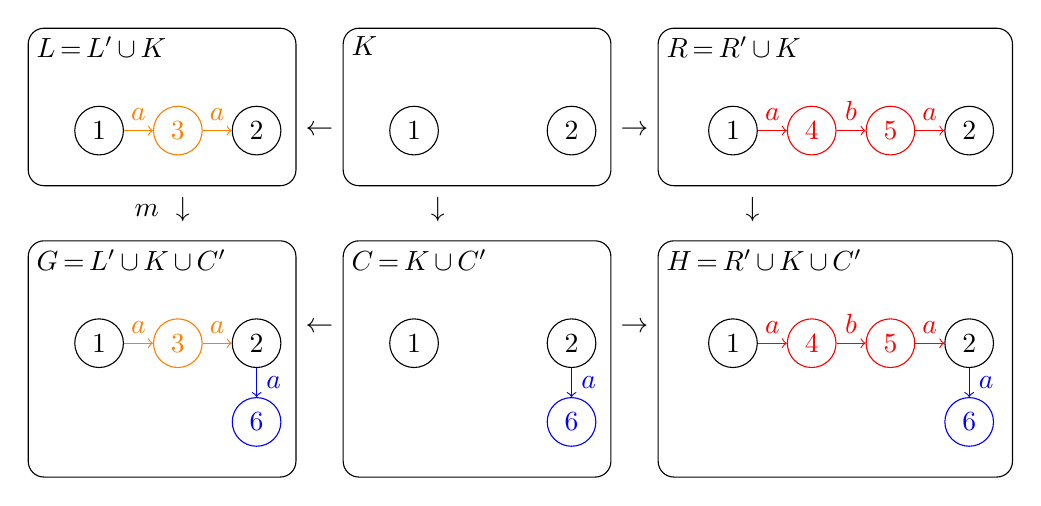
\begin{tikzpicture}
              \graphbox{\( L \mathop{=} L' \mathop{\cup} K \)}{0mm}{5mm}{34mm}{20mm}{2mm}{-5mm}{
                  \coordinate (o) at (0mm,-8mm); 
                  \node[draw,circle] (l1) at ($(o)+(-10mm,0mm)$) {1};
                  \node[draw,circle] (l2) at ($(l1)+(2,0)$) {2};
                  \node[orange,draw,circle] (l3) at ($(l1)+(1,0)$) {3};
                  \draw[orange,->] (l1) -- (l3) node[midway,above] {$a$};
                  \draw[orange,->] (l3) -- (l2) node[midway,above] {$a$};
              } 

              \graphbox{\( K \)}{40mm}{5mm}{34mm}{20mm}{2mm}{-5mm}{
                  \coordinate (o) at (0mm,-8mm); 
                  \node[draw,circle] (l1) at ($(o)+(-10mm,0mm)$) {1};
                  \node[draw,circle] (l2) at ($(l1)+(2,0)$) {2};
              }  

              \graphbox{\( R \mathop{=} R' \mathop{\cup} K \)}{80mm}{5mm}{45mm}{20mm}{2mm}{-5mm}{
                  \coordinate (o) at (-5mm,-8mm); 
                  \node[draw,circle] (l1) at ($(o)+(-10mm,0mm)$) {1};
                  \node[draw,circle] (l2) at ($(l1)+(3,0)$) {2};
                  \node[red,draw,circle] (l3) at ($(l1)+(1,0)$) {4};
                  \node[red,draw,circle] (l4) at ($(l1)+(2,0)$) {5};
                  \draw[red,->] (l1) -- (l3) node[midway,above] {$a$};
                  \draw[red,->] (l3) -- (l4) node[midway,above] {$b$};
                  \draw[red,->] (l4) -- (l2) node[midway,above] {$a$};
              }    

              \graphbox{\( G \mathop{=} L' \mathop{\cup} K \mathop{\cup} C' \)}{0mm}{-22mm}{34mm}{30mm}{2mm}{-10mm}{
                  \coordinate (o) at (0mm,-3mm); 
                  \node[draw,circle] (l1) at ($(o)+(-10mm,0mm)$) {1};
                  \node[draw,circle] (l2) at ($(l1)+(2,0)$) {2};
                  \node[draw,circle,orange] (l3) at ($(l1)+(1,0)$) {3};
                  \node[blue, draw,circle] (l4) at ($(l2)+(0,-1)$) {6};
                  \draw[orange,->] (l1) -- (l3) node[midway,above] {$a$};
                  \draw[orange,->] (l3) -- (l2) node[midway,above] {$a$};
                  \draw[blue,->] (l2) -- (l4) node[midway,right] {$a$};
                %   \node[blue,draw,circle] (l6) at ($(l1)+(0,-1)$) {7};
                %   \draw[blue,<-] (l1) -- (l6) node[midway,left] {$a$};
              }    

              \graphbox{\( C \mathop{=} K \mathop{\cup} C' \)}{40mm}{-22mm}{34mm}{30mm}{2mm}{-10mm}{
                  \coordinate (o) at (0mm,-3mm); 
                  \node[draw,circle] (l1) at ($(o)+(-10mm,0mm)$) {1};
                  \node[draw,circle] (l2) at ($(l1)+(2,0)$) {2};
                  \node[blue,draw,circle] (l4) at ($(l2)+(0,-1)$) {6};
                  \draw[blue,->] (l2) -- (l4) node[midway,right] {$a$};
                %   \node[blue,draw,circle] (l6) at ($(l1)+(0,-1)$) {7};
                %   \draw[blue,<-] (l1) -- (l6) node[midway,left] {$a$};
              }    

              \graphbox{\( H \mathop{=} R' \mathop{\cup} K \mathop{\cup} C' \)}{80mm}{-22mm}{45mm}{30mm}{2mm}{-10mm}{
                  \coordinate (o) at (-5mm,-3mm); 
                  \node[draw,circle] (l1) at ($(o)+(-10mm,0mm)$) {1};
                  \node[draw,circle] (l2) at ($(l1)+(3,0)$) {2};
                  \node[draw,circle,red] (l3) at ($(l1)+(1,0)$) {4};
                  \node[draw,circle,red] (l4) at ($(l1)+(2,0)$) {5};
                  \node[blue,draw,circle] (l5) at ($(l2)+(0,-1)$) {6};
                %   \node[blue,draw,circle] (l6) at ($(l1)+(0,-1)$) {7};
                %   \draw[blue,<-] (l1) -- (l6) node[midway,left] {$a$};
                  \draw[red,->] (l1) -- (l3) node[midway,above] {$a$};
                  \draw[red,->] (l3) -- (l4) node[midway,above] {$b$};
                  \draw[red,->] (l4) -- (l2) node[midway,above] {$a$};
                  \draw[blue,->] (l2) -- (l5) node[midway,right] {$a$};
              }    

              \node () at (37mm,-8mm) {\( \leftarrow \)}; % K -> L
              \node () at (77mm,-8mm) {\( \rightarrow \)}; % K -> R
              \node () at (17mm,-18mm) {\( m\ \downarrow \)};
              \node () at (37mm,-33mm) {\( \leftarrow \)};
              \node () at (52mm,-18mm) {\( \downarrow \)};
              \node () at (92mm,-18mm) {\( \downarrow \)};
              \node () at (77mm,-33mm) {\( \rightarrow \)}; % C -> H
      \end{tikzpicture}
      }
   \end{center}
\end{frame}


% \begin{frame}{Example} 
%  \begin{center}
%     \resizebox{0.8\textwidth}{!}{
%       \begin{tikzpicture}
%               \graphbox{\( L \mathop{=} L' \mathop{\cup} K \)}{0mm}{5mm}{34mm}{20mm}{2mm}{-5mm}{
%                   \coordinate (o) at (0mm,-8mm); 
%                   \node[draw,circle] (l1) at ($(o)+(-10mm,0mm)$) {1};
%                   \node[draw,circle] (l2) at ($(l1)+(2,0)$) {2};
%                   \node[orange,draw,circle] (l3) at ($(l1)+(1,0)$) {3};
%                   \draw[orange,->] (l1) -- (l3) node[midway,above] {$a$};
%                   \draw[orange,->] (l3) -- (l2) node[midway,above] {$a$};
%               } 

%               \graphbox{\( K \)}{40mm}{5mm}{34mm}{20mm}{2mm}{-5mm}{
%                   \coordinate (o) at (0mm,-8mm); 
%                   \node[draw,circle] (l1) at ($(o)+(-10mm,0mm)$) {1};
%                   \node[draw,circle] (l2) at ($(l1)+(2,0)$) {2};
%               }  

%               \graphbox{\( R \mathop{=} R' \mathop{\cup} K \)}{80mm}{5mm}{45mm}{20mm}{2mm}{-5mm}{
%                   \coordinate (o) at (-5mm,-8mm); 
%                   \node[draw,circle] (l1) at ($(o)+(-10mm,0mm)$) {1};
%                   \node[draw,circle] (l2) at ($(l1)+(3,0)$) {2};
%                   \node[red,draw,circle] (l3) at ($(l1)+(1,0)$) {4};
%                   \node[red,draw,circle] (l4) at ($(l1)+(2,0)$) {5};
%                   \draw[red,->] (l1) -- (l3) node[midway,above] {$a$};
%                   \draw[red,->] (l3) -- (l4) node[midway,above] {$b$};
%                   \draw[red,->] (l4) -- (l2) node[midway,above] {$a$};
%               }    

%               \graphbox{\( G \mathop{=} L' \mathop{\cup} K \mathop{\cup} C' \)}{0mm}{-22mm}{34mm}{30mm}{2mm}{-10mm}{
%                   \coordinate (o) at (0mm,-3mm); 
%                   \node[draw,circle] (l1) at ($(o)+(-10mm,0mm)$) {1};
%                   \node[draw,circle] (l2) at ($(l1)+(2,0)$) {2};
%                   \node[draw,circle,orange] (l3) at ($(l1)+(1,0)$) {3};
%                   \node[blue, draw,circle] (l4) at ($(l2)+(0,-1)$) {6};
%                   \draw[orange,->] (l1) -- (l3) node[midway,above] {$a$};
%                   \draw[orange,->] (l3) -- (l2) node[midway,above] {$a$};
%                   \draw[blue,->] (l2) -- (l4) node[midway,right] {$a$};
%                 %   \node[blue,draw,circle] (l6) at ($(l1)+(0,-1)$) {7};
%                 %   \draw[blue,<-] (l1) -- (l6) node[midway,left] {$a$};
%               }    

%               \graphbox{\( C \mathop{=} K \mathop{\cup} C' \)}{40mm}{-22mm}{34mm}{30mm}{2mm}{-10mm}{
%                   \coordinate (o) at (0mm,-3mm); 
%                   \node[draw,circle] (l1) at ($(o)+(-10mm,0mm)$) {1};
%                   \node[draw,circle] (l2) at ($(l1)+(2,0)$) {2};
%                   \node[blue,draw,circle] (l4) at ($(l2)+(0,-1)$) {6};
%                   \draw[blue,->] (l2) -- (l4) node[midway,right] {$a$};
%                 %   \node[blue,draw,circle] (l6) at ($(l1)+(0,-1)$) {7};
%                 %   \draw[blue,<-] (l1) -- (l6) node[midway,left] {$a$};
%               }    

%               \graphbox{\( H \mathop{=} R' \mathop{\cup} K \mathop{\cup} C' \)}{80mm}{-22mm}{45mm}{30mm}{2mm}{-10mm}{
%                   \coordinate (o) at (-5mm,-3mm); 
%                   \node[draw,circle] (l1) at ($(o)+(-10mm,0mm)$) {1};
%                   \node[draw,circle] (l2) at ($(l1)+(3,0)$) {2};
%                   \node[draw,circle,red] (l3) at ($(l1)+(1,0)$) {4};
%                   \node[draw,circle,red] (l4) at ($(l1)+(2,0)$) {5};
%                   \node[blue,draw,circle] (l5) at ($(l2)+(0,-1)$) {6};
%                 %   \node[blue,draw,circle] (l6) at ($(l1)+(0,-1)$) {7};
%                 %   \draw[blue,<-] (l1) -- (l6) node[midway,left] {$a$};
%                   \draw[red,->] (l1) -- (l3) node[midway,above] {$a$};
%                   \draw[red,->] (l3) -- (l4) node[midway,above] {$b$};
%                   \draw[red,->] (l4) -- (l2) node[midway,above] {$a$};
%                   \draw[blue,->] (l2) -- (l5) node[midway,right] {$a$};
%               }    

%               \node () at (37mm,-8mm) {\( \leftarrow \)}; % K -> L
%               \node () at (77mm,-8mm) {\( \rightarrow \)}; % K -> R
%               \node () at (17mm,-18mm) {\( m\ \downarrow \)};
%               \node () at (37mm,-33mm) {\( \leftarrow \)};
%               \node () at (52mm,-18mm) {\( \downarrow \)};
%               \node () at (92mm,-18mm) {\( \downarrow \)};
%               \node () at (77mm,-33mm) {\( \rightarrow \)}; % C -> H
%       \end{tikzpicture}
%       }
%    \end{center}

% %     \begin{center}
% %     \resizebox{0.7\textwidth}{!}{
% %             \begin{tikzpicture} 
% %                 \coordinate (k) at (0, 0);
% %                 \draw[fill=white] ($(k)+(0,0)$) rectangle ($(k)+(0.5,0.5)$);
% %                 \node () at ($(k)+(0.25,0.25)$) {\( \mathrm{K} \)};
            
% %                 \coordinate (c) at (0, -2.2);
% %                 \draw[fill=blue!20]
% %                 ($(c)+(0,-0.5)$)
% %                 -- ($(c)+(0,0.5)$) 
% %                 -- ($(c)+(1,0.5)$) 
% %                 arc[start angle=0, end angle=-90, radius=1]
% %                 -- cycle;
% %                 \node () at ($(c)+(0.75,0.25)$) {\( \mathrm{C'} \)};
% %                 \draw[fill=white] ($(c)+(0,0)$) rectangle ($(c)+(0.5,0.5)$);
% %                 \node () at ($(c)+(0.25,0.25)$) {\( \mathrm{K} \)};
            
% %                 \coordinate (l) at (-3, 0);
% %                 \draw[fill=orange!20] ($(l)+(-0.5,0)$) rectangle ($(l)+(0.5,1)$);
% %                 \node () at ($(l)+(-0.23,0.25)$) {\( \mathrm{L'} \)};
% %                 \draw[fill=white] ($(l)+(0,0)$) rectangle ($(l)+(0.5,0.5)$);
% %                 \node () at ($(l)+(0.25,0.25)$) {\( \mathrm{K} \)};
            
% %                 \coordinate (g) at (-3, -2.2);
% %                 \draw[fill=blue!20]
% %                 ($(g)+(0,-0.5)$)
% %                 -- ($(g)+(0,0.5)$)
% %                 -- ($(g)+(1,0.5)$) 
% %                 arc[start angle=0, end angle=-90, radius=1]
% %                 -- cycle;
% %                 \draw[fill=orange!20] ($(g)+(-0.5,0)$) rectangle ($(g)+(0.5,1)$);
% %                 \node () at ($(g)+(0.75,0.25)$) {\( \mathrm{C'} \)};
% %                 \node () at ($(g)+(-0.23,0.25)$) {\( \mathrm{L'} \)};
% %                 \draw[fill=white] ($(g)+(0,0)$) rectangle ($(g)+(0.5,0.5)$);
% %                 \node () at ($(g)+(0.25,0.25)$) {\( \mathrm{K} \)};
            
% %                 \coordinate (r) at (3,0);
% %                 \draw[fill=red!20] ($(r)+(-0.5,0)$)
% %                 -- ($(r)+(-0.5,0.5)$)
% %                 -- ($(r)+(0,1)$)
% %                 --  ($(r)+(0.5,1)$)
% %                 -- ($(r)+(0.5,0)$)
% %                 -- cycle;
% %                 \node () at ($(r)+(-0.23,0.25)$) {\( \mathrm{R'} \)};
% %                 \draw[fill=white] ($(r)+(0,0)$) rectangle ($(r)+(0.5,0.5)$);
% %                 \node () at ($(r)+(0.25,0.25)$) {\( \mathrm{K} \)};
            
% %                 \coordinate (h) at (3, -2.2);
% %                 \draw[fill=blue!20]
% %                 ($(h)+(0,-0.5)$)
% %                 -- ($(h)+(0,0.5)$)
% %                 -- ($(h)+(1,0.5)$) 
% %                 arc[start angle=0, end angle=-90, radius=1]
% %                 -- cycle;
% %                 \draw[fill=red!20] ($(h)+(-0.5,0)$)
% %                 -- ($(h)+(-0.5,0.5)$)
% %                 -- ($(h)+(0,1)$)
% %                 --  ($(h)+(0.5,1)$)
% %                 -- ($(h)+(0.5,0)$)
% %                 -- cycle;
% %             \node () at ($(h)+(0.75,0.25)$) {\( \mathrm{C'} \)};
% %             \draw[fill=white] ($(h)+(0,0)$) rectangle ($(h)+(0.5,0.5)$);
% %             \node () at ($(h)+(0.25,0.25)$) {\( \mathrm{K} \)};
% %             \node () at ($(h)+(-0.23,0.25)$) {\( \mathrm{R'} \)};
            
% %                 \node[ font=\huge] (kl) at ($(k)!0.5!(l)+(0.25,0.25)$)
% %             %    {\( \overset{l}{\leftarrow} \)}
% %                 {\( \leftarrow \)}
% %                 ; 
% %                 \node[ font=\huge] (kr) at ($(k)!0.5!(r)+(0.25,0.25)$)
% %                 {\( \rightarrow \)}
% %                 ;  
% %                 \node[ font=\huge] (cg) at ($(c)!0.5!(g)+(0.25,0.25)$) 
% %                 {\( \leftarrow \)}
% %             ;  
% %                 \node[ font=\huge] (ch) at ($(c)!0.5!(h)+(0.25,0.25)$)
% %                 {\( \rightarrow \)}
% %             ; 
% %                 \node[ font=\huge] (kc) at ($(k)!0.5!(c)+(0.2,0.4)$) {\( \downarrow \)}; 
% %             %   \node[ font=\LARGE] () at ($(l)!0.5!(g)+(0.5,0.4)$) {$m$}; 
% %                 \node[ font=\huge] (lg) at ($(l)!0.5!(g)+(0.1,0.4)$) {\( \downarrow \)}; 
% %                 \node[ font=\huge] (rh) at ($(r)!0.5!(h)+(0.1,0.4)$) {\( \downarrow \)}; 
% %             %   \node[ font=\LARGE] () at ($(r)!0.5!(h)+(0.55,0.4)$) {$m'$}; 
% %             %   \node[ font=\LARGE] () at ($(k)!0.5!(c)+(0.5,0.4)$) {$u$}; 
% %             \end{tikzpicture}
% %           }
% %    \end{center}
   
% \end{frame}

% \begin{frame}{Implicit, Explicit and Shared Occurrences}
%     An \textcolor{red}{$X$-occurrence} in a graph $G$ is an injective morphism $x: X \to G$.
%  \begin{center}
%        \resizebox{0.40\textwidth}{!}{
%         \begin{tikzpicture}
%             % [node distance=15mm]
%             \node (I) at (0,0) {$K$};
%             \node (L)  at (-2,0) {$L$};
%             \node (R)  at (2,0) {$R$};
%             \node (G)  at (-2,-2) {$G$};
%             \node (C)  at (0,-2) {$C$};
%             \node (H)  at (2,-2) {$H$};
%             \draw [->] (I) to  node [midway,below] { } (L);
%             \draw [->] (I) to  node [midway,below] { } (R);
%             \draw [->] (L) to node [midway,right] { } (G);
%             \draw [->] (I) to  node [midway,right] 
%             % {$u$}
%             {} (C);
%             \draw [->] (R) to  node [midway,right] 
%             {}
%             (H);
%             \draw [->] (C) to node [midway,above] {} (G);
%             \draw [->] (C) to node [midway,above] 
%             {}
%             (H);
%             % \node [at=($(I)!.5!(G)$)] {\normalfont PO};
%             % \node [at=($(I)!.5!(H)$)] {\normalfont PO};
%         \end{tikzpicture}
%     }
%     \resizebox{0.40\textwidth}{!}{
%             \begin{tikzpicture} 
%                 \coordinate (k) at (0, 0);
%                 \draw[fill=white] ($(k)+(0,0)$) rectangle ($(k)+(0.5,0.5)$);
%                 \node () at ($(k)+(0.25,0.25)$) {\( \mathrm{K} \)};
            
%                 \coordinate (c) at (0, -2.2);
%                 \draw[fill=blue!20]
%                 ($(c)+(0,-0.5)$)
%                 -- ($(c)+(0,0.5)$) 
%                 -- ($(c)+(1,0.5)$) 
%                 arc[start angle=0, end angle=-90, radius=1]
%                 -- cycle;
%                 \node () at ($(c)+(0.75,0.25)$) {\( \mathrm{C'} \)};
%                 \draw[fill=white] ($(c)+(0,0)$) rectangle ($(c)+(0.5,0.5)$);
%                 \node () at ($(c)+(0.25,0.25)$) {\( \mathrm{K} \)};
            
%                 \coordinate (l) at (-3, 0);
%                 \draw[fill=orange!20] ($(l)+(-0.5,0)$) rectangle ($(l)+(0.5,1)$);
%                 \node () at ($(l)+(-0.23,0.25)$) {\( \mathrm{L'} \)};
%                 \draw[fill=white] ($(l)+(0,0)$) rectangle ($(l)+(0.5,0.5)$);
%                 \node () at ($(l)+(0.25,0.25)$) {\( \mathrm{K} \)};
            
%                 \coordinate (g) at (-3, -2.2);
%                 \draw[fill=blue!20]
%                 ($(g)+(0,-0.5)$)
%                 -- ($(g)+(0,0.5)$)
%                 -- ($(g)+(1,0.5)$) 
%                 arc[start angle=0, end angle=-90, radius=1]
%                 -- cycle;
%                 \draw[fill=orange!20] ($(g)+(-0.5,0)$) rectangle ($(g)+(0.5,1)$);
%                 \node () at ($(g)+(0.75,0.25)$) {\( \mathrm{C'} \)};
%                 \node () at ($(g)+(-0.23,0.25)$) {\( \mathrm{L'} \)};
%                 \draw[fill=white] ($(g)+(0,0)$) rectangle ($(g)+(0.5,0.5)$);
%                 \node () at ($(g)+(0.25,0.25)$) {\( \mathrm{K} \)};
            
%                 \coordinate (r) at (3,0);
%                 \draw[fill=red!20] ($(r)+(-0.5,0)$)
%                 -- ($(r)+(-0.5,0.5)$)
%                 -- ($(r)+(0,1)$)
%                 --  ($(r)+(0.5,1)$)
%                 -- ($(r)+(0.5,0)$)
%                 -- cycle;
%                 \node () at ($(r)+(-0.23,0.25)$) {\( \mathrm{R'} \)};
%                 \draw[fill=white] ($(r)+(0,0)$) rectangle ($(r)+(0.5,0.5)$);
%                 \node () at ($(r)+(0.25,0.25)$) {\( \mathrm{K} \)};
            
%                 \coordinate (h) at (3, -2.2);
%                 \draw[fill=blue!20]
%                 ($(h)+(0,-0.5)$)
%                 -- ($(h)+(0,0.5)$)
%                 -- ($(h)+(1,0.5)$) 
%                 arc[start angle=0, end angle=-90, radius=1]
%                 -- cycle;
%                 \draw[fill=red!20] ($(h)+(-0.5,0)$)
%                 -- ($(h)+(-0.5,0.5)$)
%                 -- ($(h)+(0,1)$)
%                 --  ($(h)+(0.5,1)$)
%                 -- ($(h)+(0.5,0)$)
%                 -- cycle;
%             \node () at ($(h)+(0.75,0.25)$) {\( \mathrm{C'} \)};
%             \draw[fill=white] ($(h)+(0,0)$) rectangle ($(h)+(0.5,0.5)$);
%             \node () at ($(h)+(0.25,0.25)$) {\( \mathrm{K} \)};
%             \node () at ($(h)+(-0.23,0.25)$) {\( \mathrm{R'} \)};
            
%                 \node[ font=\huge] (kl) at ($(k)!0.5!(l)+(0.25,0.25)$)
%             %    {\( \overset{l}{\leftarrow} \)}
%                 {\( \leftarrow \)}
%                 ; 
%                 \node[ font=\huge] (kr) at ($(k)!0.5!(r)+(0.25,0.25)$)
%                 {\( \rightarrow \)}
%                 ;  
%                 \node[ font=\huge] (cg) at ($(c)!0.5!(g)+(0.25,0.25)$) 
%                 {\( \leftarrow \)}
%             ;  
%                 \node[ font=\huge] (ch) at ($(c)!0.5!(h)+(0.25,0.25)$)
%                 {\( \rightarrow \)}
%             ; 
%                 \node[ font=\huge] (kc) at ($(k)!0.5!(c)+(0.2,0.4)$) {\( \downarrow \)}; 
%             %   \node[ font=\LARGE] () at ($(l)!0.5!(g)+(0.5,0.4)$) {$m$}; 
%                 \node[ font=\huge] (lg) at ($(l)!0.5!(g)+(0.1,0.4)$) {\( \downarrow \)}; 
%                 \node[ font=\huge] (rh) at ($(r)!0.5!(h)+(0.1,0.4)$) {\( \downarrow \)}; 
%             %   \node[ font=\LARGE] () at ($(r)!0.5!(h)+(0.55,0.4)$) {$m'$}; 
%             %   \node[ font=\LARGE] () at ($(k)!0.5!(c)+(0.5,0.4)$) {$u$}; 
%             \end{tikzpicture}
%           }
%    \end{center}

%    An $X$-occurrence $x: X \to G$ is 
%    \begin{itemize}
%     \item \textcolor{red}{shared} if 
%     $\opn{Im(x)}$ is included in $C$;
%     \item \textcolor{red}{explicit} if 
%     $\opn{Im(x)}$ is included in $L$;
%     \item \textcolor{red}{implicit} if 
%     $\opn{Im(x)}$ has elements in both $C'$ and $L'$.
%    \end{itemize}

%    Similarly, in $H$.
%     % An $X$-occurrence $x: X \to G$ is 

%     % \parbox{0.45\textwidth}{\hspace{3mm}$\bullet$ 
%     % \textcolor{red}{shared} if 
%     % $\opn{Im(x)}$ is included in $C$
%     % }

%     % \parbox{0.45\textwidth}{\hspace{3mm}$\bullet$ 
%     % \textcolor{red}{explicit} if 
%     % $\opn{Im(x)}$ is included in $L$
%     % }

%     % \parbox{\textwidth}{\hspace{3mm}$\bullet$ 
%     % \textcolor{red}{implicit} if 
%     % $\opn{Im(x)}$ has elements in both $C'$ and $L'$
%     % }
% %     $X$-occurrence $x: X \to H$ is 

% %    \parbox{0.45\textwidth}{\hspace{3mm}$\bullet$ 
% %    \textcolor{red}{shared} if 
% %     $\opn{Im(x)}$ is included in $C$ 
% %    }
   
% %    \parbox{0.45\textwidth}{\hspace{3mm}$\bullet$ \textcolor{red}{explicit} if 
% %     $\opn{Im(x)}$ is included in $R$
% %    }

% %     \parbox{\textwidth}{\hspace{3mm}$\bullet$ \textcolor{red}{implicit} if 
% %     $\opn{Im(x)}$ has elements in both $C'$ and $R'$
% %     }
% \end{frame}


\begin{frame}{Implicit, Explicit and Shared Occurrences}
    An \textcolor{red}{$X$-occurrence} in a graph $G$ is an injective morphism $x: X \to G$.
 \begin{center}
    \resizebox{0.5\textwidth}{!}{
            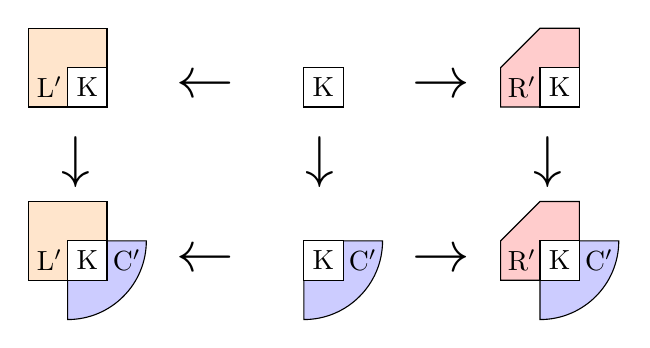
\begin{tikzpicture} 
                \coordinate (k) at (0, 0);
                \draw[fill=white] ($(k)+(0,0)$) rectangle ($(k)+(0.5,0.5)$);
                \node () at ($(k)+(0.25,0.25)$) {\( \mathrm{K} \)};
            
                \coordinate (c) at (0, -2.2);
                \draw[fill=blue!20]
                ($(c)+(0,-0.5)$)
                -- ($(c)+(0,0.5)$) 
                -- ($(c)+(1,0.5)$) 
                arc[start angle=0, end angle=-90, radius=1]
                -- cycle;
                \node () at ($(c)+(0.75,0.25)$) {\( \mathrm{C'} \)};
                \draw[fill=white] ($(c)+(0,0)$) rectangle ($(c)+(0.5,0.5)$);
                \node () at ($(c)+(0.25,0.25)$) {\( \mathrm{K} \)};
            
                \coordinate (l) at (-3, 0);
                \draw[fill=orange!20] ($(l)+(-0.5,0)$) rectangle ($(l)+(0.5,1)$);
                \node () at ($(l)+(-0.23,0.25)$) {\( \mathrm{L'} \)};
                \draw[fill=white] ($(l)+(0,0)$) rectangle ($(l)+(0.5,0.5)$);
                \node () at ($(l)+(0.25,0.25)$) {\( \mathrm{K} \)};
            
                \coordinate (g) at (-3, -2.2);
                \draw[fill=blue!20]
                ($(g)+(0,-0.5)$)
                -- ($(g)+(0,0.5)$)
                -- ($(g)+(1,0.5)$) 
                arc[start angle=0, end angle=-90, radius=1]
                -- cycle;
                \draw[fill=orange!20] ($(g)+(-0.5,0)$) rectangle ($(g)+(0.5,1)$);
                \node () at ($(g)+(0.75,0.25)$) {\( \mathrm{C'} \)};
                \node () at ($(g)+(-0.23,0.25)$) {\( \mathrm{L'} \)};
                \draw[fill=white] ($(g)+(0,0)$) rectangle ($(g)+(0.5,0.5)$);
                \node () at ($(g)+(0.25,0.25)$) {\( \mathrm{K} \)};
            
                \coordinate (r) at (3,0);
                \draw[fill=red!20] ($(r)+(-0.5,0)$)
                -- ($(r)+(-0.5,0.5)$)
                -- ($(r)+(0,1)$)
                --  ($(r)+(0.5,1)$)
                -- ($(r)+(0.5,0)$)
                -- cycle;
                \node () at ($(r)+(-0.23,0.25)$) {\( \mathrm{R'} \)};
                \draw[fill=white] ($(r)+(0,0)$) rectangle ($(r)+(0.5,0.5)$);
                \node () at ($(r)+(0.25,0.25)$) {\( \mathrm{K} \)};
            
                \coordinate (h) at (3, -2.2);
                \draw[fill=blue!20]
                ($(h)+(0,-0.5)$)
                -- ($(h)+(0,0.5)$)
                -- ($(h)+(1,0.5)$) 
                arc[start angle=0, end angle=-90, radius=1]
                -- cycle;
                \draw[fill=red!20] ($(h)+(-0.5,0)$)
                -- ($(h)+(-0.5,0.5)$)
                -- ($(h)+(0,1)$)
                --  ($(h)+(0.5,1)$)
                -- ($(h)+(0.5,0)$)
                -- cycle;
            \node () at ($(h)+(0.75,0.25)$) {\( \mathrm{C'} \)};
            \draw[fill=white] ($(h)+(0,0)$) rectangle ($(h)+(0.5,0.5)$);
            \node () at ($(h)+(0.25,0.25)$) {\( \mathrm{K} \)};
            \node () at ($(h)+(-0.23,0.25)$) {\( \mathrm{R'} \)};
            
                \node[ font=\huge] (kl) at ($(k)!0.5!(l)+(0.25,0.25)$)
            %    {\( \overset{l}{\leftarrow} \)}
                {\( \leftarrow \)}
                ; 
                \node[ font=\huge] (kr) at ($(k)!0.5!(r)+(0.25,0.25)$)
                {\( \rightarrow \)}
                ;  
                \node[ font=\huge] (cg) at ($(c)!0.5!(g)+(0.25,0.25)$) 
                {\( \leftarrow \)}
            ;  
                \node[ font=\huge] (ch) at ($(c)!0.5!(h)+(0.25,0.25)$)
                {\( \rightarrow \)}
            ; 
                \node[ font=\huge] (kc) at ($(k)!0.5!(c)+(0.2,0.4)$) {\( \downarrow \)}; 
            %   \node[ font=\LARGE] () at ($(l)!0.5!(g)+(0.5,0.4)$) {$m$}; 
                \node[ font=\huge] (lg) at ($(l)!0.5!(g)+(0.1,0.4)$) {\( \downarrow \)}; 
                \node[ font=\huge] (rh) at ($(r)!0.5!(h)+(0.1,0.4)$) {\( \downarrow \)}; 
            %   \node[ font=\LARGE] () at ($(r)!0.5!(h)+(0.55,0.4)$) {$m'$}; 
            %   \node[ font=\LARGE] () at ($(k)!0.5!(c)+(0.5,0.4)$) {$u$}; 
            \end{tikzpicture}
          }
   \end{center}

   An $X$-occurrence $x: X \to G$ is 
   \begin{itemize}
    \item \textcolor{red}{explicit} if 
        $\opn{Im(x)}$ is included in 
            \resizebox{0.1\textwidth}{!}{
                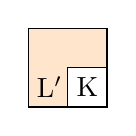
\begin{tikzpicture}
                    \coordinate (l) at (-3, 0);
                    \draw[fill=orange!20] ($(l)+(-0.5,0)$) rectangle ($(l)+(0.5,1)$);
                    \node () at ($(l)+(-0.23,0.25)$) {\( \mathrm{L'} \)};
                    \draw[fill=white] ($(l)+(0,0)$) rectangle ($(l)+(0.5,0.5)$);
                    \node () at ($(l)+(0.25,0.25)$) {\( \mathrm{K} \)};
                \end{tikzpicture}
            }
    \item \textcolor{red}{shared} if 
        $\opn{Im(x)}$ is included in 
            \resizebox{0.1\textwidth}{!}{
                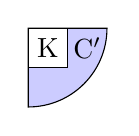
\begin{tikzpicture} 
                    \coordinate (c) at (0, -2.2);
                    \draw[fill=blue!20]
                    ($(c)+(0,-0.5)$)
                    -- ($(c)+(0,0.5)$) 
                    -- ($(c)+(1,0.5)$) 
                    arc[start angle=0, end angle=-90, radius=1]
                    -- cycle;
                    \node () at ($(c)+(0.75,0.25)$) {\( \mathrm{C'} \)};
                    \draw[fill=white] ($(c)+(0,0)$) rectangle ($(c)+(0.5,0.5)$);
                    \node () at ($(c)+(0.25,0.25)$) {\( \mathrm{K} \)};
                \end{tikzpicture}
            }
    \item \textcolor{red}{implicit} if 
        $\opn{Im(x)}$ has elements in both 
            \resizebox{0.1\textwidth}{!}{
                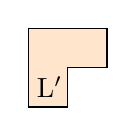
\begin{tikzpicture}
                    \coordinate (g) at (-3, -2.2);
                    \draw[fill=orange!20] ($(g)+(-0.5,0)$) rectangle ($(g)+(0.5,1)$);
                    \node () at ($(g)+(-0.23,0.25)$) {\( \mathrm{L'} \)};
                    \draw[fill=white] ($(g)+(0,0)$) rectangle ($(g)+(0.5,0.5)$);
                    \draw[white,very thick] (-3, -2.2) -- (-2.5, -2.2) --  (-2.5, -1.7);
                \end{tikzpicture}
            } and 
            \resizebox{0.1\textwidth}{!}{
                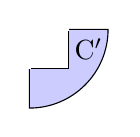
\begin{tikzpicture}
                    \coordinate (g) at (-3, -2.2);
                    \draw[fill=blue!20]
                    ($(g)+(0,-0.5)$)
                    -- ($(g)+(0,0.5)$)
                    -- ($(g)+(1,0.5)$) 
                    arc[start angle=0, end angle=-90, radius=1]
                    -- cycle;
                    \node () at ($(g)+(0.75,0.25)$) {\( \mathrm{C'} \)};
                    \draw[fill=white] ($(g)+(0,0)$) rectangle ($(g)+(0.5,0.5)$);
                    \draw[white,very thick]  (-3.0, -2.2) -- (-3.0, -1.7) -- (-2.5, -1.7);
                \end{tikzpicture}
            }
   \end{itemize}

   Similarly, in $H$.
\end{frame}
 

\begin{frame}{Example}
Let $X$ be the graph 
\tikz[baseline=-0.5ex]{ 
        \node (x) at (0,0) {$\bullet$};  
        \node (y) at (1,0) {$\bullet$};
        \node (z) at (2,0) {$\bullet$};
        \draw[->] (x) -- node[midway,below] {$a$} (y) ;
        \draw[->] (y) -- node[midway,below] {$a$} (z) ;
}. Consider the rewriting step:
  \begin{center}
        \resizebox{0.7\textwidth}{!}{
      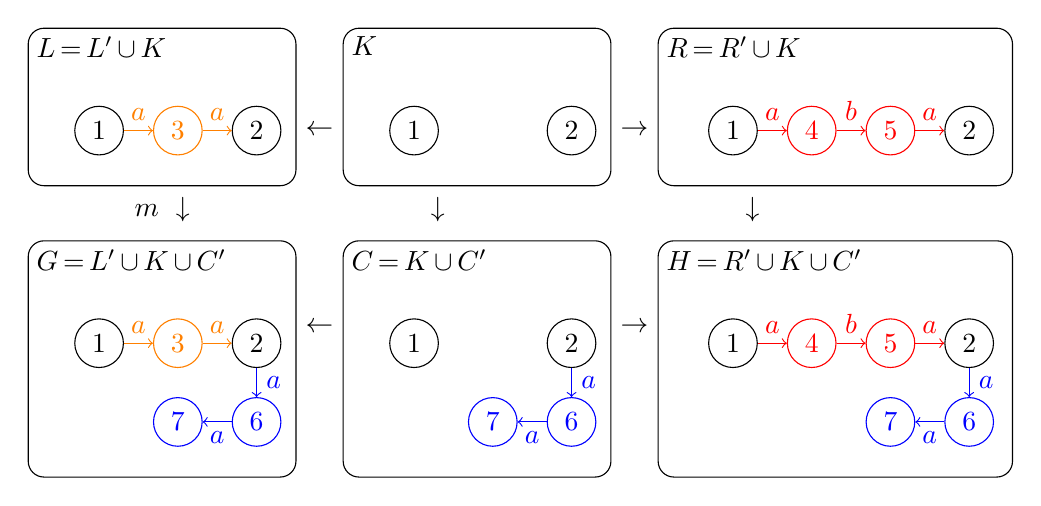
\begin{tikzpicture}
              \graphbox{\( L \mathop{=} L' \mathop{\cup} K \)}{0mm}{5mm}{34mm}{20mm}{2mm}{-5mm}{
                  \coordinate (o) at (0mm,-8mm); 
                  \node[draw,circle] (l1) at ($(o)+(-10mm,0mm)$) {1};
                  \node[draw,circle] (l2) at ($(l1)+(2,0)$) {2};
                  \node[orange,draw,circle] (l3) at ($(l1)+(1,0)$) {3};
                  \draw[orange,->] (l1) -- (l3) node[midway,above] {$a$};
                  \draw[orange,->] (l3) -- (l2) node[midway,above] {$a$};
              } 

              \graphbox{\( K \)}{40mm}{5mm}{34mm}{20mm}{2mm}{-5mm}{
                  \coordinate (o) at (0mm,-8mm); 
                  \node[draw,circle] (l1) at ($(o)+(-10mm,0mm)$) {1};
                  \node[draw,circle] (l2) at ($(l1)+(2,0)$) {2};
              }  

              \graphbox{\( R \mathop{=} R' \mathop{\cup} K \)}{80mm}{5mm}{45mm}{20mm}{2mm}{-5mm}{
                  \coordinate (o) at (-5mm,-8mm); 
                  \node[draw,circle] (l1) at ($(o)+(-10mm,0mm)$) {1};
                  \node[draw,circle] (l2) at ($(l1)+(3,0)$) {2};
                  \node[red,draw,circle] (l3) at ($(l1)+(1,0)$) {4};
                  \node[red,draw,circle] (l4) at ($(l1)+(2,0)$) {5};
                  \draw[red,->] (l1) -- (l3) node[midway,above] {$a$};
                  \draw[red,->] (l3) -- (l4) node[midway,above] {$b$};
                  \draw[red,->] (l4) -- (l2) node[midway,above] {$a$};
              }    

              \graphbox{\( G \mathop{=} L' \mathop{\cup} K \mathop{\cup} C' \)}{0mm}{-22mm}{34mm}{30mm}{2mm}{-10mm}{
                  \coordinate (o) at (0mm,-3mm); 
                  \node[draw,circle] (l1) at ($(o)+(-10mm,0mm)$) {1};
                  \node[draw,circle] (l2) at ($(l1)+(2,0)$) {2};
                  \node[draw,circle,orange] (l3) at ($(l1)+(1,0)$) {3};
                  \node[blue, draw,circle] (l4) at ($(l2)+(0,-1)$) {6};
                  \draw[orange,->] (l1) -- (l3) node[midway,above] {$a$};
                  \draw[orange,->] (l3) -- (l2) node[midway,above] {$a$};
                  \draw[blue,->] (l2) -- (l4) node[midway,right] {$a$};
                %   \node[blue,draw,circle] (l6) at ($(l1)+(0,-1)$) {7};
                %   \draw[blue,<-] (l1) -- (l6) node[midway,left] {$a$};
                \node[blue,draw,circle] (l7) at ($(l4)+(-1,0)$) {7};
                  \draw[blue,->] (l4) -- (l7) node[midway,below] {$a$};
              }    

              \graphbox{\( C \mathop{=} K \mathop{\cup} C' \)}{40mm}{-22mm}{34mm}{30mm}{2mm}{-10mm}{
                  \coordinate (o) at (0mm,-3mm); 
                  \node[draw,circle] (l1) at ($(o)+(-10mm,0mm)$) {1};
                  \node[draw,circle] (l2) at ($(l1)+(2,0)$) {2};
                  \node[blue,draw,circle] (l4) at ($(l2)+(0,-1)$) {6};
                  \draw[blue,->] (l2) -- (l4) node[midway,right] {$a$};
                %   \node[blue,draw,circle] (l6) at ($(l1)+(0,-1)$) {7};
                %   \draw[blue,<-] (l1) -- (l6) node[midway,left] {$a$};
                    \node[blue,draw,circle] (l7) at ($(l4)+(-1,0)$) {7};
                  \draw[blue,->] (l4) -- (l7) node[midway,below] {$a$};
              }    

              \graphbox{\( H \mathop{=} R' \mathop{\cup} K \mathop{\cup} C' \)}{80mm}{-22mm}{45mm}{30mm}{2mm}{-10mm}{
                  \coordinate (o) at (-5mm,-3mm); 
                  \node[draw,circle] (l1) at ($(o)+(-10mm,0mm)$) {1};
                  \node[draw,circle] (l2) at ($(l1)+(3,0)$) {2};
                  \node[draw,circle,red] (l3) at ($(l1)+(1,0)$) {4};
                  \node[draw,circle,red] (l4) at ($(l1)+(2,0)$) {5};
                  \node[blue,draw,circle] (l5) at ($(l2)+(0,-1)$) {6};
                %   \node[blue,draw,circle] (l6) at ($(l1)+(0,-1)$) {7};
                %   \draw[blue,<-] (l1) -- (l6) node[midway,left] {$a$};
                  \draw[red,->] (l1) -- (l3) node[midway,above] {$a$};
                  \draw[red,->] (l3) -- (l4) node[midway,above] {$b$};
                  \draw[red,->] (l4) -- (l2) node[midway,above] {$a$};
                  \draw[blue,->] (l2) -- (l5) node[midway,right] {$a$};
                        \node[blue,draw,circle] (l7) at ($(l5)+(-1,0)$) {7};
                  \draw[blue,->] (l5) -- (l7) node[midway,below] {$a$};
              }    

              \node () at (37mm,-8mm) {\( \leftarrow \)}; % K -> L
              \node () at (77mm,-8mm) {\( \rightarrow \)}; % K -> R
              \node () at (17mm,-18mm) {\( m\ \downarrow \)};
              \node () at (37mm,-33mm) {\( \leftarrow \)};
              \node () at (52mm,-18mm) {\( \downarrow \)};
              \node () at (92mm,-18mm) {\( \downarrow \)};
              \node () at (77mm,-33mm) {\( \rightarrow \)}; % C -> H
      \end{tikzpicture}
        }
    \end{center}

 Explicit $X$-occurrence in $G$:
    \resizebox{0.18\textwidth}{!}{  
        \tikz[baseline=-0.5ex]{ 
            \node[draw,circle] (x) at (0,0) {1};  
            \node[orange,draw,circle] (y) at (1,0) {3};
            \node[draw,circle] (z) at (2,0) {2};
            \draw[orange,->] (x) -- node[midway,above] {$a$} (y) ;
            \draw[orange,->] (y) -- node[midway,above] {$a$} (z) ;
        }
    }
 
     Explicit $X$-occurrence in $H$: None.

   Implicit $X$-occurrences in $G$:
     \resizebox{0.18\textwidth}{!}{
        \tikz[baseline=-0.5ex]{ 
            \node[orange,draw,circle] (x) at (0,0) {3};  
            \node[draw,circle] (y) at (1,0) {2};
            \node[blue,draw,circle] (z) at (2,0) {6};
            \draw[orange,->] (x) -- node[midway,above] {$a$} (y) ;
            \draw[blue,->] (y) -- node[midway,above] {$a$} (z) ;
        } 
    }

   Implicit $X$-occurrence in $H$: 
    \resizebox{0.18\textwidth}{!}{
        \tikz[baseline=-0.5ex]{ 
            \node[red,draw,circle] (x) at (0,0) {5};  
            \node[draw,circle] (y) at (1,0) {2};
            \node[blue,draw,circle] (z) at (2,0) {6};
            \draw[red,->] (x) -- node[midway,above] {$a$} (y) ;
            \draw[blue,->] (y) -- node[midway,above] {$a$} (z) ;
        }
    }

      Shared $X$-occurrence by $G$ and $H$: 
    \resizebox{0.18\textwidth}{!}{
        \tikz[baseline=-0.5ex]{ 
            \node[draw,circle] (x) at (0,0) {2};  
            \node[blue,draw,circle] (y) at (1,0) {6};
            \node[blue,draw,circle] (z) at (2,0) {7};
            \draw[blue,->] (x) -- node[midway,above] {$a$} (y) ;
            \draw[blue,->] (y) -- node[midway,above] {$a$} (z) ;
        }
    }

    Obersvation: Shared $X$-occurrences in $G$ and $H$ are the same. 
\end{frame}
\subsection{Challenges in establishing a sufficient condition for termination}
\begin{frame}{A sufficient condition for termination}
    %     \begin{flalign*}
    %         &\mathop{\mid}\text{$X$-occurrences in $G$}\mathop{\mid} - \mathop{\mid}\text{$X$-occurrences in $H$}\mathop{\mid} \\
    %         =&(\mathop{\mid}\text{explicit $X$-occurrences in $G$}\mathop{\mid} \mathop{-} \mathop{\mid}\text{explicit $X$-occurrences in $H$}\mathop{\mid})  \mathop{+}\\
    %                 &(\mathop{\mid}\text{implicit $X$-occurrences in $G$}\mathop{\mid} \mathop{-} \mathop{\mid}\text{implicit $X$-occurrences in $H$}\mathop{\mid})
    %         \end{flalign*} 
            $\varphi$ terminates if for all rewriting step:
            \begin{center}
       \resizebox{0.40\textwidth}{!}{
        \begin{tikzpicture}
            % [node distance=15mm]
            \node (I) at (0,0) {$K$};
            \node (L)  at (-2,0) {$L$};
            \node (R)  at (2,0) {$R$};
            \node (G)  at (-2,-2) {$G$};
            \node (C)  at (0,-2) {$C$};
            \node (H)  at (2,-2) {$H$};
            \draw [->] (I) to  node [midway,below] { } (L);
            \draw [->] (I) to  node [midway,below] { } (R);
            \draw [->] (L) to node [midway,right] { } (G);
            \draw [->] (I) to  node [midway,right] 
            % {$u$}
            {} (C);
            \draw [->] (R) to  node [midway,right] 
            {}
            (H);
            \draw [->] (C) to node [midway,above] {} (G);
            \draw [->] (C) to node [midway,above] 
            {}
            (H);
            % \node [at=($(I)!.5!(G)$)] {\normalfont PO};
            % \node [at=($(I)!.5!(H)$)] {\normalfont PO};
        \end{tikzpicture}
    }
    \end{center}
            the following holds:
        \begin{enumerate}
            \item $|\text{explicit $X$-occurrences in $G$}| 
                    \mathop{>} 
                    |\text{explicit $X$-occurrences in $H$}|$;
            \item $|\text{implicit $X$-occurrences in $G$}|
                    \mathop{\geq} 
                    |\text{implicit $X$-occurrences in $H$}|$.
        \end{enumerate}

    The \textcolor{red}{first condition}
    \textcolor{red}{is straightforward} because
    \begin{itemize}
        \item $\text{explicit $X$-occurrences in $G$}$ = $\text{$X$-occurrences in $L$}$,  
        \item $\text{explicit $X$-occurrences in $H$}$ = $\text{$X$-occurrences in $R$}$,  
        \item $|\text{$X$-occurrences in $L$}|$ and $|\text{$X$-occurrences in $R$}|$ are computable.
    \end{itemize}

    Challenge: Establishing the \textcolor{red}{second condition}.
\end{frame} 

\subsection{A solution}

\begin{frame}{Analysis of Implicit Occurrences in $G$ and $H$}
         \begin{center} 
        \resizebox{0.9\textwidth}{!}{
        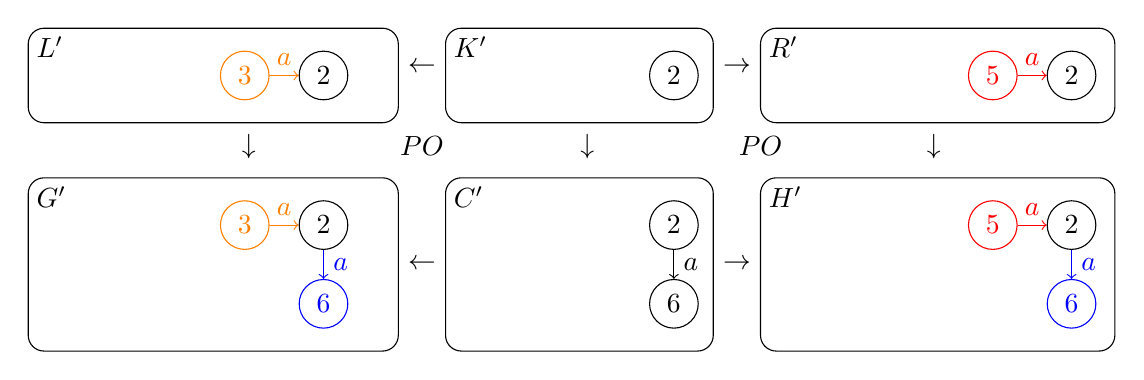
\begin{tikzpicture}
            \graphbox{\( L' \)}{-13mm}{-3mm}{47mm}{12mm}{2mm}{2mm}{
                \coordinate (o) at (2mm,-8mm); 
                \node[circle] (l1) at ($(o)+(-10mm,0mm)$) {};
                \node[draw,circle] (l2) at ($(l1)+(2,0)$) {2};
                \node[orange,draw,circle] (l3) at ($(l1)+(1,0)$) {3};
                \draw[orange,->] (l3) -- (l2) node[midway,above] {$a$};
            } 
     
            \graphbox{\( R' \)}{80mm}{-3mm}{45mm}{12mm}{2mm}{2mm}{
                \coordinate (o) at (-5mm,-8mm); 
                \node[circle] (l1) at ($(o)+(-10mm,0mm)$) {};
                \node[draw,circle] (l2) at ($(l1)+(3,0)$) {2};
                \node[red,draw,circle] (l4) at ($(l1)+(2,0)$) {5};
                \draw[red,->] (l4) -- (l2) node[midway,above] {$a$};
            }    
     
            \graphbox{\( G'\)}{-13mm}{-22mm}{47mm}{22mm}{2mm}{-3mm}{
                \coordinate (o) at (2mm,-3mm); 
                \node[circle] (l1) at ($(o)+(-10mm,0mm)$) {};
                \node[draw,circle] (l2) at ($(l1)+(2,0)$) {2};
                \node[orange,draw,circle] (l3) at ($(l1)+(1,0)$) {3};
                \node[blue,draw,circle] (l4) at ($(l2)+(0,-1)$) {6};
                \draw[orange,->] (l3) -- (l2) node[midway,above] {$a$};
                \draw[blue,->] (l2) -- (l4) node[midway,right] {$a$};
            }    
    
            \graphbox{\( K' \)}{40mm}{-3mm}{34mm}{12mm}{2mm}{2mm}{
                \coordinate (o) at (0mm,-8mm); 
                \node[circle] (l1) at ($(o)+(-10mm,0mm)$) {};
                \node[draw,circle] (l2) at ($(l1)+(2,0)$) {2};
            } 
            \graphbox{\( C'  \)}{40mm}{-22mm}{34mm}{22mm}{2mm}{-3mm}{
                \coordinate (o) at (0mm,-3mm); 
                \node[circle] (l1) at ($(o)+(-10mm,0mm)$) {};
                \node[draw,circle] (l2) at ($(l1)+(2,0)$) {2};
                \node[draw,circle] (l4) at ($(l2)+(0,-1)$) {6};
                \draw[->] (l2) -- (l4) node[midway,right] {$a$};
            }  
    
            \graphbox{\( H' \)}{80mm}{-22mm}{45mm}{22mm}{2mm}{-3mm}{
                \coordinate (o) at (-5mm,-3mm); 
                \node[circle] (l1) at ($(o)+(-10mm,0mm)$) {};
                \node[draw,circle] (l2) at ($(l1)+(3,0)$) {2};
                \node[circle] (l3) at ($(l1)+(1,0)$) {};
                \node[red,draw,circle] (l4) at ($(l1)+(2,0)$) {5};
                \node[blue,draw,circle] (l5) at ($(l2)+(0,-1)$) {6};
                \node[circle] (l6) at ($(l1)+(0,-1)$) {};
                \draw[red,->] (l4) -- (l2) node[midway,above] {$a$};
                \draw[blue,->] (l2) -- (l5) node[midway,right] {$a$};
            }    
             
            \node () at (37mm,-8mm) {\( \leftarrow \)}; % K -> L
            \node () at (77mm,-8mm) {\( \rightarrow \)}; % K -> R
            \node () at (15mm,-18mm) {\(\downarrow \)};
            \node () at (37mm,-33mm) {\( \leftarrow \)};
            \node () at (37mm,-18mm) {$PO$};
            \node () at (58mm,-18mm) {\( \downarrow \)};
            \node () at (80mm,-18mm) {$PO$};
            \node () at (102mm,-18mm) {\( \downarrow \)};
            \node () at (77mm,-33mm) {\( \rightarrow \)}; % C -> H
        \end{tikzpicture}
        }         
    \end{center}

        The occurrence is $C' \mathop{\cup} R'$. \resizebox{0.18\textwidth}{!}{
        \tikz[baseline=-0.5ex]{ 
            \node[draw,circle] (y) at (1,0) {2};
            \node[blue,draw,circle] (z) at (2,0) {6};
            \draw[blue,->] (y) -- node[midway,above] {$a$} (z) ;
        } 
    } is shared by $G$ and $H$. 
     \resizebox{0.18\textwidth}{!}{
        \tikz[baseline=-0.5ex]{ 
            \node[red,draw,circle] (x) at (0,0) {5};  
            \node[draw,circle] (y) at (1,0) {2};
            \draw[red,->] (x) -- node[midway,above] {$a$} (y) ;
        }
    }
    is not in $G$ but there is 
    \resizebox{0.18\textwidth}{!}{
        \tikz[baseline=-0.5ex]{ 
            \node[orange,draw,circle] (x) at (0,0) {3};  
            \node[draw,circle] (y) at (1,0) {2};
            \draw[orange,->] (x) -- node[midway,above] {$a$} (y) ;
        } 
    }
    in $G$ and $C' \mathop{\cup} L'$ is an implicit occurrence in $G$.
\end{frame}

\begin{frame}{$X$-non-increasing rule}
    Let $\varphi: L \mathop{\leftarrow} K \mathop{\rightarrow} R$ be a rule.
        \begin{lemma}[More $X$-occurrences before rewriting]
        For all $G \mathop{\Rightarrow}_\varphi H$, there are more implicit $X$-occurrences in $G$ than in $H$, if 

        \enquote{subgraphs of $R$ that can form an implicit $X$-occurrence in some rewriting step can be mapped to subgraphs in $L$ while 
    preserving the interface elements}.

    \end{lemma}
\end{frame}
% \begin{frame}
%  \begin{center}
%        \resizebox{0.49\textwidth}{!}{
%         \begin{tikzpicture}
%             % [node distance=15mm]
%             \node (I) at (0,0) {$K$};
%             \node (L)  at (-2,0) {$L$};
%             \node (R)  at (2,0) {$R$};
%             \node (G)  at (-2,-2) {$G$};
%             \node (C)  at (0,-2) {$C$};
%             \node (H)  at (2,-2) {$H$};
%             \draw [->] (I) to  node [midway,below] { } (L);
%             \draw [->] (I) to  node [midway,below] { } (R);
%             \draw [->] (L) to node [midway,right] { } (G);
%             \draw [->] (I) to  node [midway,right] 
%             % {$u$}
%             {} (C);
%             \draw [->] (R) to  node [midway,right] 
%             {$m'$}
%             (H);
%             \draw [->] (C) to node [midway,above] {} (G);
%             \draw [->] (C) to node [midway,above] 
%             {}
%             (H);
%             % \node [at=($(I)!.5!(G)$)] {\normalfont PO};
%             % \node [at=($(I)!.5!(H)$)] {\normalfont PO};
%         \end{tikzpicture}
%     }
%     \resizebox{0.49\textwidth}{!}{
%             \begin{tikzpicture} 
%                 \coordinate (k) at (0, 0);
%                 \draw[fill=white] ($(k)+(0,0)$) rectangle ($(k)+(0.5,0.5)$);
%                 \node () at ($(k)+(0.25,0.25)$) {\( \mathrm{K} \)};
            
%                 \coordinate (c) at (0, -2.2);
%                 \draw[fill=blue!20]
%                 ($(c)+(0,-0.5)$)
%                 -- ($(c)+(0,0.5)$) 
%                 -- ($(c)+(1,0.5)$) 
%                 arc[start angle=0, end angle=-90, radius=1]
%                 -- cycle;
%                 \node () at ($(c)+(0.75,0.25)$) {\( \mathrm{C'} \)};
%                 \draw[fill=white] ($(c)+(0,0)$) rectangle ($(c)+(0.5,0.5)$);
%                 \node () at ($(c)+(0.25,0.25)$) {\( \mathrm{K} \)};
            
%                 \coordinate (l) at (-3, 0);
%                 \draw[fill=orange!20] ($(l)+(-0.5,0)$) rectangle ($(l)+(0.5,1)$);
%                 \node () at ($(l)+(-0.23,0.25)$) {\( \mathrm{L'} \)};
%                 \draw[fill=white] ($(l)+(0,0)$) rectangle ($(l)+(0.5,0.5)$);
%                 \node () at ($(l)+(0.25,0.25)$) {\( \mathrm{K} \)};
            
%                 \coordinate (g) at (-3, -2.2);
%                 \draw[fill=blue!20]
%                 ($(g)+(0,-0.5)$)
%                 -- ($(g)+(0,0.5)$)
%                 -- ($(g)+(1,0.5)$) 
%                 arc[start angle=0, end angle=-90, radius=1]
%                 -- cycle;
%                 \draw[fill=orange!20] ($(g)+(-0.5,0)$) rectangle ($(g)+(0.5,1)$);
%                 \node () at ($(g)+(0.75,0.25)$) {\( \mathrm{C'} \)};
%                 \node () at ($(g)+(-0.23,0.25)$) {\( \mathrm{L'} \)};
%                 \draw[fill=white] ($(g)+(0,0)$) rectangle ($(g)+(0.5,0.5)$);
%                 \node () at ($(g)+(0.25,0.25)$) {\( \mathrm{K} \)};
            
%                 \coordinate (r) at (3,0);
%                 \draw[fill=red!20] ($(r)+(-0.5,0)$)
%                 -- ($(r)+(-0.5,0.5)$)
%                 -- ($(r)+(0,1)$)
%                 --  ($(r)+(0.5,1)$)
%                 -- ($(r)+(0.5,0)$)
%                 -- cycle;
%                 \node () at ($(r)+(-0.23,0.25)$) {\( \mathrm{R'} \)};
%                 \draw[fill=white] ($(r)+(0,0)$) rectangle ($(r)+(0.5,0.5)$);
%                 \node () at ($(r)+(0.25,0.25)$) {\( \mathrm{K} \)};
            
%                 \coordinate (h) at (3, -2.2);
%                 \draw[fill=blue!20]
%                 ($(h)+(0,-0.5)$)
%                 -- ($(h)+(0,0.5)$)
%                 -- ($(h)+(1,0.5)$) 
%                 arc[start angle=0, end angle=-90, radius=1]
%                 -- cycle;
%                 \draw[fill=red!20] ($(h)+(-0.5,0)$)
%                 -- ($(h)+(-0.5,0.5)$)
%                 -- ($(h)+(0,1)$)
%                 --  ($(h)+(0.5,1)$)
%                 -- ($(h)+(0.5,0)$)
%                 -- cycle;
%             \node () at ($(h)+(0.75,0.25)$) {\( \mathrm{C'} \)};
%             \draw[fill=white] ($(h)+(0,0)$) rectangle ($(h)+(0.5,0.5)$);
%             \node () at ($(h)+(0.25,0.25)$) {\( \mathrm{K} \)};
%             \node () at ($(h)+(-0.23,0.25)$) {\( \mathrm{R'} \)};
            
%                 \node[ font=\huge] (kl) at ($(k)!0.5!(l)+(0.25,0.25)$)
%             %    {\( \overset{l}{\leftarrow} \)}
%                 {\( \leftarrow \)}
%                 ; 
%                 \node[ font=\huge] (kr) at ($(k)!0.5!(r)+(0.25,0.25)$)
%                 {\( \rightarrow \)}
%                 ;  
%                 \node[ font=\huge] (cg) at ($(c)!0.5!(g)+(0.25,0.25)$) 
%                 {\( \leftarrow \)}
%             ;  
%                 \node[ font=\huge] (ch) at ($(c)!0.5!(h)+(0.25,0.25)$)
%                 {\( \rightarrow \)}
%             ; 
%                 \node[ font=\huge] (kc) at ($(k)!0.5!(c)+(0.2,0.4)$) {\( \downarrow \)}; 
%             %   \node[ font=\LARGE] () at ($(l)!0.5!(g)+(0.5,0.4)$) {$m$}; 
%                 \node[ font=\huge] (lg) at ($(l)!0.5!(g)+(0.1,0.4)$) {\( \downarrow \)}; 
%                 \node[ font=\huge] (rh) at ($(r)!0.5!(h)+(0.1,0.4)$) {\( \downarrow \)}; 
%             %   \node[ font=\LARGE] () at ($(r)!0.5!(h)+(0.55,0.4)$) {$m'$}; 
%             %   \node[ font=\LARGE] () at ($(k)!0.5!(c)+(0.5,0.4)$) {$u$}; 
%             \end{tikzpicture}
%           }
%    \end{center}

%    Implicit $X$-occurrence $x$ in $G$ is of form $L_x \mathop{\cup} C'_x$ 
     
%    Implicit $X$-occurrence $x$ in $G$ is of form $R_x \mathop{\cup} C'_x$
    
%     It suffices to map different $R_x$ to different $L_x$ in such a way that 
%     \begin{itemize}
%         \item there is an injection from implicit $X$-occurrences in $H$ to implicit $X$-occurrences in $G$ 
%     \end{itemize}
% \end{frame}


% \begin{frame}{The set $D(R,X)$ of all subgraphs of $R$ that can form an implicitly created $X$-occurrence in some rewriting step}
%     % $D(L,X)$ : set of all subgraphs of $L$ that can form an implicitly deleted $X$-occurrence in some rewriting step
%     Example:
%      \begin{center}
%         \resizebox{\textwidth}{!}{ 
%             \begin{tikzpicture}
%                 \graphbox{$L$}{0mm}{0mm}{35mm}{35mm}{2mm}{-5mm}{
%                     \coordinate (delta) at (0,-18mm);
%                     \node[draw,circle] (l1) at ($(delta)+(-1,1.5)$) {1};
%                     \node[draw,circle] (l2) at ($(delta)+(1,1.5)$) {2};
%                     \node[draw,circle] (l3) at ($(delta)+(0,0)$) {3};
%                     \draw[->] (l1) -- (l3) node[midway,left] {$s$};
%                     \draw[->] (l2) -- (l3) node[midway,right] {$s$};
%                     \draw[->] (l3) edge [loop below] node {0} (l3);
%                 }
%                     \graphbox{$K$}{40mm}{0mm}{35mm}{35mm}{2mm}{-5mm}{
%                         \coordinate (delta) at (0,-18mm);
%                         \coordinate (interfaceorigin) at ($(delta) +(5,0)$);
%                         \node[draw,circle] (r1) at ($(delta) +(-1,1.5)$) {1};
%                         \node[draw,circle] (r2) at ($(delta) +(0.5,1.5)$) {2};
%                         \node[draw,circle] (r3) at ($(delta)+(0,0)$) {3};
%                         % \draw[->] (r1) -- (r3) node[midway,left] {$s$};
%                         % \draw[->] (r3) edge [loop below] node {0} (r3);
%                     } 
%                     \node () at (38mm,-18mm) {$\leftarrow$};
%                     \node () at (77mm,-18mm) {$\rightarrow$};
%                 \graphbox{$R$}{80mm}{0mm}{50mm}{35mm}{2mm}{-5mm}{
%                     \coordinate (delta) at (-10mm,-18mm);
%                     \node[draw,circle] (r1) at ($(delta)+(-1,1.5)$) {1};
%                     \node[draw,circle] (r2) at ($(delta)+(0.5,1.5)$) {2};
%                     \node[draw,circle] (r3) at ($(delta)+(0,0)$) {3};
%                     \node[draw,circle] (r4) at ($(delta)+(1,0)$) {};
%                     \draw[->] (r1) -- (r3) node[midway,left] {$s$};
%                     \draw[->] (r2) -- (r4) node[midway,right] {$s$};
%                     \draw[->] (r4) edge [loop below] node {0} (r4);
%                     \draw[->] (r3) edge [loop below] node {0} (r3);
%                     \node[draw,circle] (r5) at ($(r2)+(1.5,0)$) {};
%                     \draw[->] (r5) edge [loop below] node {0} (r5);
%                     \draw[->] (r5) edge [loop right] node {0} (r5);
%                     \draw[->] (r5) edge [loop left] node {0} (r5);
%                 }
%                 % \graphbox{$R_x$}{40mm}{40mm}{35mm}{35mm}{2mm}{-5mm}{
%                 %     \coordinate (delta) at (0,-18mm);
%                 %     \coordinate (rxorigin) at ($(interfaceorigin)+(0,6)$);
%                 %     \node[draw,circle] (r1) at ($(delta)+(-1,1.5)$) {1};
%                 %     \node[draw,circle] (r2) at ($(delta)\mathop{+} (0.5,1.5)$) {2};
%                 %     \node[draw,circle] (r3) at ($(delta)\mathop{+} (0,0)$) {3};
%                 %     \draw[->] (r1) -- (r3) node[midway,left] {$s$};
%                 %     % \draw[->] (r3) edge [loop below] node {0} (r3);
%                 % }
                
%                 % \node () at (57mm,2mm) {$\uparrowtail$};
%                 % \node () at (38mm,2mm) {$\swarrowtail$};
%                 % \node () at (79mm,2mm) {$\searrowtail$};
%             \end{tikzpicture}
%             }
%     \end{center}

%     $X$ : the graph $\tikz[baseline=-0.5ex]{ 
%                 \node (x) at (0,0) {$\bullet$}; 
%                 \node (y) at (1,0) {$\bullet$};
%                 \node (z) at (2,0) {$\bullet$};
%                 \draw[->] (x) -- (y) node[midway, above] {$s$};
%                 \draw[->] (z) -- (y) node[midway, above] {$s$};
%         }$

%     % $D(L,X)$: $L'_1$:
%     %     \raisebox{2pt}{
%     %         \scalebox{0.7}{\tikz[baseline=-0.5ex]{
%     %         \node [draw,circle] (x) at (0,0) {1};
%     %         \node[draw,circle] (y) at (1,0) {3};
%     %         \draw[->] (x) -- (y) node[midway, above] {$s$};
%     %     }}}, $L'_2$:
%     %     \raisebox{2pt}{
%     %         \scalebox{0.7}{\tikz[baseline=-0.5ex]{
%     %         \node [draw,circle] (z) at (2,0) {2};
%     %         \node [draw,circle] (x) at (0,0) {1};
%     %         \node[draw,circle] (y) at (1,0) {3};
%     %         \draw[->] (x) -- (y) node[midway, above] {$s$};
%     %     }}}, 
%     %     $L'_3$:
%     %     \raisebox{2pt}{
%     %         \scalebox{0.7}{\tikz[baseline=-0.5ex]{
%     %         \node [draw,circle] (z) at (2,0) {2};
%     %         \node [draw,circle] (y) at (1,0) {3};
%     %         \draw[->] (z) -- (y) node[midway, above] {$s$};
%     %     }}},
%     %     $L'_4$:
%     %     \raisebox{2pt}{
%     %         \scalebox{0.7}{\tikz[baseline=-0.5ex]{
%     %         \node [draw,circle] (z) at (2,0) {2};
%     %         \node [draw,circle] (x) at (0,0) {1};
%     %         \node[draw,circle] (y) at (1,0) {3};
%     %         \draw[->] (z) -- (y) node[midway, above] {$s$};
%     %     }}}

%     $D(R,X)$ consists of $R_1$:
%         \raisebox{2pt}{
%             \scalebox{0.7}{\tikz[baseline=-0.5ex]{
%             \node [draw,circle] (x) at (0,0) {1};
%             \node[draw,circle] (y) at (1,0) {3};
%             \draw[->] (x) -- (y) node[midway, above] {$s$};
%         }}} and $R_2$:
%         \raisebox{2pt}{
%             \scalebox{0.7}{\tikz[baseline=-0.5ex]{
%             \node [draw,circle] (z) at (2,0) {2};
%             \node [draw,circle] (x) at (0,0) {1};
%             \node[draw,circle] (y) at (1,0) {3};
%             \draw[->] (x) -- (y) node[midway, above] {$s$};
%         }}}
% \end{frame}

\begin{frame}{Example}
    Rewriting rule:
     \begin{center} 
            \resizebox{\textwidth}{!}{
           \begin{tikzpicture}
                \graphbox{\( L \)}{0mm}{-3mm}{34mm}{12mm}{2mm}{2mm}{
                    \coordinate (o) at (0mm,-8mm); 
                    \node[draw,circle] (l1) at ($(o)+(-10mm,0mm)$) {1};
                    \node[draw,circle] (l2) at ($(l1)+(2,0)$) {2};
                    \node[draw,circle] (l3) at ($(l1)+(1,0)$) {};
                    \draw[->] (l1) -- (l3) node[midway,above] {$a$};
                    \draw[->] (l3) -- (l2) node[midway,above] {$a$};
                } 
        
                \graphbox{\( K \)}{40mm}{-3mm}{34mm}{12mm}{2mm}{2mm}{
                    \coordinate (o) at (0mm,-8mm); 
                    \node[draw,circle] (l1) at ($(o)+(-10mm,0mm)$) {1};
                    \node[draw,circle] (l2) at ($(l1)+(2,0)$) {2};
                }  
        
                \graphbox{\( R \)}{80mm}{-3mm}{45mm}{12mm}{2mm}{2mm}{
                    \coordinate (o) at (-5mm,-8mm); 
                    \node[draw,circle] (l1) at ($(o)+(-10mm,0mm)$) {1};
                    \node[draw,circle] (l2) at ($(l1)+(3,0)$) {2};
                    \node[draw,circle] (l3) at ($(l1)+(1,0)$) {4};
                    \node[draw,circle] (l4) at ($(l1)+(2,0)$) {5};
                    \draw[->] (l1) -- (l3) node[midway,above] {$a$};
                    \draw[->] (l3) -- (l4) node[midway,above] {$b$};
                    \draw[->] (l4) -- (l2) node[midway,above] {$a$};
                }    
                \node () at (37mm,-8mm) {\( \overset{l}{\leftarrow} \)}; % K -> L
                \node () at (77mm,-8mm) {\( \overset{r}{\rightarrow} \)}; % K -> R
            \end{tikzpicture}
            }         
        \end{center}
    The set $D(R,X)$ of subgraphs of $R$ which can form an implicit $X$-occurrence in some rewriting step:
    \begin{center}  
        \resizebox{\textwidth}{!}{
        
\begin{tikzpicture}     
            \graphbox{\( R'_1 \)}{80mm}{-3mm}{45mm}{12mm}{2mm}{2mm}{
                \coordinate (o) at (-5mm,-8mm); 
                \node[circle] (l1) at ($(o)+(-10mm,0mm)$) {};
                \node[draw,circle] (l2) at ($(l1)+(3,0)$) {2};
                \node[draw,circle] (l4) at ($(l1)+(2,0)$) {5};
                \draw[->] (l4) -- (l2) node[midway,above] {$a$};
            } 
            \phantom{
                \graphbox{\( K'_1 \)}{40mm}{-3mm}{34mm}{12mm}{2mm}{2mm}{
                    \coordinate (o) at (0mm,-8mm); 
                    \node[circle] (l1) at ($(o)+(-10mm,0mm)$) {};
                    \node[draw,circle] (l2) at ($(l1)+(2,0)$) {2};
                }
                \graphbox{$L$}{133mm}{-3mm}{34mm}{12mm}{2mm}{2mm}{
                    \coordinate (o) at (0mm,-8mm); 
                    \node[draw,circle] (l1) at ($(o)+(-10mm,0mm)$) {};
                    \node[draw,circle] (l2) at ($(l1)+(2,0)$) {2};
                    \node[draw,circle] (l3) at ($(l1)+(1,0)$) {5};
                    \draw[->] (l1) -- (l3) node[midway,above] {$a$};
                    \draw[->] (l3) -- (l2) node[midway,above] {$a$};
                }
                \node () at (129mm,-8mm) {\(\overset{\textcolor{red}{h_1}}{\rightarrow}\)};
                \node () at (77mm,-8mm) {\( \rightarrow \)}; 
            }
        \end{tikzpicture}
        }         
    \end{center}

    \begin{center} 
        \resizebox{\textwidth}{!}{
        
\begin{tikzpicture}
            \graphbox{\( R_2' \)}{80mm}{-3mm}{45mm}{12mm}{2mm}{2mm}{
                \coordinate (o) at (-5mm,-8mm); 
                \node[draw,circle] (l1) at ($(o)+(-10mm,0mm)$) {1};
                \node[draw,circle] (l2) at ($(l1)+(3,0)$) {2};
                \node[draw,circle] (l4) at ($(l1)+(2,0)$) {5};
                \draw[->] (l4) -- (l2) node[midway,above] {$a$};
            }     
            \phantom{
                \graphbox{\( K'_2  \)}{40mm}{-3mm}{34mm}{12mm}{2mm}{2mm}{
                \coordinate (o) at (0mm,-8mm); 
                \node[draw,circle] (l1) at ($(o)+(-10mm,0mm)$) {1};
                \node[draw,circle] (l2) at ($(l1)+(2,0)$) {2};
                }
                \graphbox{$L$}{133mm}{-3mm}{34mm}{12mm}{2mm}{2mm}{
                    \coordinate (o) at (0mm,-8mm); 
                    \node[draw,circle] (l1) at ($(o)+(-10mm,0mm)$) {1};
                    \node[draw,circle] (l2) at ($(l1)+(2,0)$) {2};
                    \node[draw,circle] (l3) at ($(l1)+(1,0)$) {5};
                    \draw[->] (l1) -- (l3) node[midway,above] {$a$};
                    \draw[->] (l3) -- (l2) node[midway,above] {$a$};
                }
                \node () at (129mm,-8mm) {\(\overset{\textcolor{red}{h_2}}{\rightarrow}\)};
                \node () at (77mm,-8mm) {\( \rightarrow \)}; 
            }
        \end{tikzpicture}
        }         
    \end{center}

    \begin{center} 
        \resizebox{\textwidth}{!}{
        \begin{tikzpicture}
            \graphbox{\( R'_3 \)}{80mm}{-3mm}{45mm}{12mm}{2mm}{2mm}{
                \coordinate (o) at (-5mm,-8mm); 
                \node[draw,circle] (l1) at ($(o)+(-10mm,0mm)$) {1};
                \node[draw,circle] (l3) at ($(l1)+(1,0)$) {4};
                \draw[->] (l1) -- (l3) node[midway,above] {$a$};
            }  
            \phantom{  
                \graphbox{\( K'_3 \)}{40mm}{-3mm}{34mm}{12mm}{2mm}{2mm}{
                    \coordinate (o) at (0mm,-8mm); 
                    \node[draw,circle] (l1) at ($(o)+(-10mm,0mm)$) {1};
                }  
                \graphbox{$L$}{133mm}{-3mm}{34mm}{12mm}{2mm}{2mm}{
                    \coordinate (o) at (0mm,-8mm); 
                    \node[draw,circle] (l1) at ($(o)+(-10mm,0mm)$) {1};
                    \node[draw,circle] (l2) at ($(l1)+(2,0)$) {};
                    \node[draw,circle] (l3) at ($(l1)+(1,0)$) {4};
                    \draw[->] (l1) -- (l3) node[midway,above] {$a$};
                    \draw[->] (l3) -- (l2) node[midway,above] {$a$};
                }
                \node () at (129mm,-8mm) {\(\overset{\textcolor{red}{h_3}}{\rightarrow}\)};
                \node () at (77mm,-8mm) {\( \rightarrow \)}; % K -> R
            }
        \end{tikzpicture}
        }         
    \end{center}

       \begin{center} 
        \resizebox{\textwidth}{!}{
        
\begin{tikzpicture}
            \graphbox{\( R'_4 \)}{80mm}{-3mm}{45mm}{12mm}{2mm}{2mm}{
                \coordinate (o) at (-5mm,-8mm); 
                \node[draw,circle] (l1) at ($(o)+(-10mm,0mm)$) {1};
                \node[draw,circle] (l2) at ($(l1)+(3,0)$) {2};
                \node[draw,circle] (l3) at ($(l1)+(1,0)$) {4};
                % \node[draw,circle] (l4) at ($(l1)+(2,0)$) {5};
                \draw[->] (l1) -- (l3) node[midway,above] {$a$};
                % \draw[->] (l3) -- (l4) node[midway,above] {$b$};
                % \draw[->] (l4) -- (l2) node[midway,above] {$a$};
            }  
            \phantom{  
                \graphbox{\( K'_4 \)}{40mm}{-3mm}{34mm}{12mm}{2mm}{2mm}{
                    \coordinate (o) at (0mm,-8mm); 
                    \node[draw,circle] (l1) at ($(o)+(-10mm,0mm)$) {1};
                    \node[draw,circle] (l2) at ($(l1)+(2,0)$) {2};
                }   
                \graphbox{$L$}{133mm}{-3mm}{34mm}{12mm}{2mm}{2mm}{
                    \coordinate (o) at (0mm,-8mm); 
                    \node[draw,circle] (l1) at ($(o)+(-10mm,0mm)$) {1};
                    \node[draw,circle] (l2) at ($(l1)+(2,0)$) {2};
                    \node[draw,circle] (l3) at ($(l1)+(1,0)$) {4};
                    \draw[->] (l1) -- (l3) node[midway,above] {$a$};
                    \draw[->] (l3) -- (l2) node[midway,above] {$a$};
                }
                \node () at (129mm,-8mm) {\(\overset{\textcolor{red}{h_4}}{\rightarrow}\)};
                \node () at (77mm,-8mm) {\( \rightarrow \)}; % K -> R
            }
        \end{tikzpicture}
        }         
    \end{center}
\end{frame}


\begin{frame}{Example}
    Rewriting rule:
 \begin{center} 
            \resizebox{\textwidth}{!}{
           \begin{tikzpicture}
                \graphbox{\( L \)}{0mm}{-3mm}{34mm}{12mm}{2mm}{2mm}{
                    \coordinate (o) at (0mm,-8mm); 
                    \node[draw,circle] (l1) at ($(o)+(-10mm,0mm)$) {1};
                    \node[draw,circle] (l2) at ($(l1)+(2,0)$) {2};
                    \node[draw,circle] (l3) at ($(l1)+(1,0)$) {};
                    \draw[->] (l1) -- (l3) node[midway,above] {$a$};
                    \draw[->] (l3) -- (l2) node[midway,above] {$a$};
                } 
        
                \graphbox{\( K \)}{40mm}{-3mm}{34mm}{12mm}{2mm}{2mm}{
                    \coordinate (o) at (0mm,-8mm); 
                    \node[draw,circle] (l1) at ($(o)+(-10mm,0mm)$) {1};
                    \node[draw,circle] (l2) at ($(l1)+(2,0)$) {2};
                }  
        
                \graphbox{\( R \)}{80mm}{-3mm}{45mm}{12mm}{2mm}{2mm}{
                    \coordinate (o) at (-5mm,-8mm); 
                    \node[draw,circle] (l1) at ($(o)+(-10mm,0mm)$) {1};
                    \node[draw,circle] (l2) at ($(l1)+(3,0)$) {2};
                    \node[draw,circle] (l3) at ($(l1)+(1,0)$) {4};
                    \node[draw,circle] (l4) at ($(l1)+(2,0)$) {5};
                    \draw[->] (l1) -- (l3) node[midway,above] {$a$};
                    \draw[->] (l3) -- (l4) node[midway,above] {$b$};
                    \draw[->] (l4) -- (l2) node[midway,above] {$a$};
                }    
                \node () at (37mm,-8mm) {\( \overset{l}{\leftarrow} \)}; % K -> L
                \node () at (77mm,-8mm) {\( \overset{r}{\rightarrow} \)}; % K -> R
            \end{tikzpicture}
            }         
        \end{center}
    Distinct graphs in $D(R,X)$ can be mapped to subgraphs in $L$ while 
    preserving the interface elements.
    \begin{center}  
        \resizebox{\textwidth}{!}{
        \begin{tikzpicture}    
            \graphbox{\( K'_1 \)}{40mm}{-3mm}{34mm}{12mm}{2mm}{2mm}{
                \coordinate (o) at (0mm,-8mm); 
                \node[circle] (l1) at ($(o)+(-10mm,0mm)$) {};
                \node[draw,circle] (l2) at ($(l1)+(2,0)$) {2};
            } 
            \graphbox{\( R'_1 \)}{80mm}{-3mm}{45mm}{12mm}{2mm}{2mm}{
                \coordinate (o) at (-5mm,-8mm); 
                \node[circle] (l1) at ($(o)+(-10mm,0mm)$) {};
                \node[draw,circle] (l2) at ($(l1)+(3,0)$) {2};
                \node[draw,circle] (l4) at ($(l1)+(2,0)$) {5};
                \draw[->] (l4) -- (l2) node[midway,above] {$a$};
            } 
            \graphbox{$L$}{133mm}{-3mm}{34mm}{12mm}{2mm}{2mm}{
                \coordinate (o) at (0mm,-8mm); 
                \node[draw,circle] (l1) at ($(o)+(-10mm,0mm)$) {};
                \node[draw,circle] (l2) at ($(l1)+(2,0)$) {2};
                \node[draw,circle] (l3) at ($(l1)+(1,0)$) {5};
                \draw[->] (l1) -- (l3) node[midway,above] {$a$};
                \draw[->] (l3) -- (l2) node[midway,above] {$a$};
            }
            \node () at (129mm,-8mm) {\(\overset{\textcolor{red}{h_1}}{\rightarrow}\)};
            \node () at (77mm,-8mm) {\( \rightarrow \)}; % K -> R
        \end{tikzpicture}
        }         
    \end{center}

    \begin{center} 
        \resizebox{\textwidth}{!}{
        \begin{tikzpicture}
            \graphbox{\( K'_2  \)}{40mm}{-3mm}{34mm}{12mm}{2mm}{2mm}{
                \coordinate (o) at (0mm,-8mm); 
                \node[draw,circle] (l1) at ($(o)+(-10mm,0mm)$) {1};
                \node[draw,circle] (l2) at ($(l1)+(2,0)$) {2};
            }  
    
            \graphbox{\( R_2' \)}{80mm}{-3mm}{45mm}{12mm}{2mm}{2mm}{
                \coordinate (o) at (-5mm,-8mm); 
                \node[draw,circle] (l1) at ($(o)+(-10mm,0mm)$) {1};
                \node[draw,circle] (l2) at ($(l1)+(3,0)$) {2};
                \node[draw,circle] (l4) at ($(l1)+(2,0)$) {5};
                \draw[->] (l4) -- (l2) node[midway,above] {$a$};
            }     
     
            \graphbox{$L$}{133mm}{-3mm}{34mm}{12mm}{2mm}{2mm}{
                \coordinate (o) at (0mm,-8mm); 
                \node[draw,circle] (l1) at ($(o)+(-10mm,0mm)$) {1};
                \node[draw,circle] (l2) at ($(l1)+(2,0)$) {2};
                \node[draw,circle] (l3) at ($(l1)+(1,0)$) {5};
                \draw[->] (l1) -- (l3) node[midway,above] {$a$};
                \draw[->] (l3) -- (l2) node[midway,above] {$a$};
            }
            \node () at (129mm,-8mm) {\(\overset{\textcolor{red}{h_2}}{\rightarrow}\)};
            \node () at (77mm,-8mm) {\( \rightarrow \)}; % K -> R
        \end{tikzpicture}
        }         
    \end{center}

    \begin{center} 
        \resizebox{\textwidth}{!}{
        \begin{tikzpicture}
            \graphbox{\( K'_3 \)}{40mm}{-3mm}{34mm}{12mm}{2mm}{2mm}{
                \coordinate (o) at (0mm,-8mm); 
                \node[draw,circle] (l1) at ($(o)+(-10mm,0mm)$) {1};
            }  
    
            \graphbox{\( R'_3 \)}{80mm}{-3mm}{45mm}{12mm}{2mm}{2mm}{
                \coordinate (o) at (-5mm,-8mm); 
                \node[draw,circle] (l1) at ($(o)+(-10mm,0mm)$) {1};
                \node[draw,circle] (l3) at ($(l1)+(1,0)$) {4};
                \draw[->] (l1) -- (l3) node[midway,above] {$a$};
            }    
            \graphbox{$L$}{133mm}{-3mm}{34mm}{12mm}{2mm}{2mm}{
                \coordinate (o) at (0mm,-8mm); 
                \node[draw,circle] (l1) at ($(o)+(-10mm,0mm)$) {1};
                \node[draw,circle] (l2) at ($(l1)+(2,0)$) {};
                \node[draw,circle] (l3) at ($(l1)+(1,0)$) {4};
                \draw[->] (l1) -- (l3) node[midway,above] {$a$};
                \draw[->] (l3) -- (l2) node[midway,above] {$a$};
            }
            \node () at (129mm,-8mm) {\(\overset{\textcolor{red}{h_3}}{\rightarrow}\)};
            \node () at (77mm,-8mm) {\( \rightarrow \)}; % K -> R
        \end{tikzpicture}
        }         
    \end{center}

       \begin{center} 
        \resizebox{\textwidth}{!}{
        \begin{tikzpicture}
            \graphbox{\( K'_4 \)}{40mm}{-3mm}{34mm}{12mm}{2mm}{2mm}{
                \coordinate (o) at (0mm,-8mm); 
                \node[draw,circle] (l1) at ($(o)+(-10mm,0mm)$) {1};
                \node[draw,circle] (l2) at ($(l1)+(2,0)$) {2};

            }  
    
            \graphbox{\( R'_4 \)}{80mm}{-3mm}{45mm}{12mm}{2mm}{2mm}{
                \coordinate (o) at (-5mm,-8mm); 
                \node[draw,circle] (l1) at ($(o)+(-10mm,0mm)$) {1};
                \node[draw,circle] (l2) at ($(l1)+(3,0)$) {2};
                \node[draw,circle] (l3) at ($(l1)+(1,0)$) {4};
                % \node[draw,circle] (l4) at ($(l1)+(2,0)$) {5};
                \draw[->] (l1) -- (l3) node[midway,above] {$a$};
                % \draw[->] (l3) -- (l4) node[midway,above] {$b$};
                % \draw[->] (l4) -- (l2) node[midway,above] {$a$};
            }    
            \graphbox{$L$}{133mm}{-3mm}{34mm}{12mm}{2mm}{2mm}{
                \coordinate (o) at (0mm,-8mm); 
                \node[draw,circle] (l1) at ($(o)+(-10mm,0mm)$) {1};
                \node[draw,circle] (l2) at ($(l1)+(2,0)$) {2};
                \node[draw,circle] (l3) at ($(l1)+(1,0)$) {4};
                \draw[->] (l1) -- (l3) node[midway,above] {$a$};
                \draw[->] (l3) -- (l2) node[midway,above] {$a$};
            }
            \node () at (129mm,-8mm) {\(\overset{\textcolor{red}{h_4}}{\rightarrow}\)};
            \node () at (77mm,-8mm) {\( \rightarrow \)}; % K -> R
        \end{tikzpicture}
        }         
    \end{center}
\end{frame}

\begin{frame}{Main Results}

         
    \begin{theorem}[Sufficient Termination Condition]
        Let $\varphi$ be a $X$-non-increasing rule.
        $\varphi$ is terminating if there are strictly more explicit $X$-occurrences in $L$ than in $R$.
    \end{theorem}

\end{frame}


\begin{frame}{Terminating of Running Example}
     \begin{center} 
            \resizebox{\textwidth}{!}{
           \begin{tikzpicture}
                \graphbox{\( L \)}{0mm}{-3mm}{34mm}{12mm}{2mm}{2mm}{
                    \coordinate (o) at (0mm,-8mm); 
                    \node[draw,circle] (l1) at ($(o)+(-10mm,0mm)$) {1};
                    \node[draw,circle] (l2) at ($(l1)+(2,0)$) {2};
                    \node[draw,circle] (l3) at ($(l1)+(1,0)$) {};
                    \draw[->] (l1) -- (l3) node[midway,above] {$a$};
                    \draw[->] (l3) -- (l2) node[midway,above] {$a$};
                } 
        
                \graphbox{\( K \)}{40mm}{-3mm}{34mm}{12mm}{2mm}{2mm}{
                    \coordinate (o) at (0mm,-8mm); 
                    \node[draw,circle] (l1) at ($(o)+(-10mm,0mm)$) {1};
                    \node[draw,circle] (l2) at ($(l1)+(2,0)$) {2};
                }  
        
                \graphbox{\( R \)}{80mm}{-3mm}{45mm}{12mm}{2mm}{2mm}{
                    \coordinate (o) at (-5mm,-8mm); 
                    \node[draw,circle] (l1) at ($(o)+(-10mm,0mm)$) {1};
                    \node[draw,circle] (l2) at ($(l1)+(3,0)$) {2};
                    \node[draw,circle] (l3) at ($(l1)+(1,0)$) {};
                    \node[draw,circle] (l4) at ($(l1)+(2,0)$) {};
                    \draw[->] (l1) -- (l3) node[midway,above] {$a$};
                    \draw[->] (l3) -- (l4) node[midway,above] {$b$};
                    \draw[->] (l4) -- (l2) node[midway,above] {$a$};
                }    
                \node () at (37mm,-8mm) {\( \overset{l}{\leftarrow} \)}; % K -> L
                \node () at (77mm,-8mm) {\( \overset{r}{\rightarrow} \)}; % K -> R
            \end{tikzpicture}
            }         
    \end{center}
    \begin{itemize}
        \item X :  \tikz[baseline=-0.5ex]{ 
        \node (x) at (0,0) {$\bullet$};  
        \node (y) at (1,0) {$\bullet$};
        \node (z) at (2,0) {$\bullet$};
        \draw[->] (x) -- node[midway,below] {$a$} (y) ;
        \draw[->] (y) -- node[midway,below] {$a$} (z) ;
        }
        \item $X$-non-increasing rule
        \item Strictly more explicit $X$-occurrences in $L$ than in $R$: $$1 \mathop{>} 0$$
    \end{itemize}
\end{frame}

\begin{frame}{Termination of Motivating Rule}
     \begin{center}
        \resizebox{\textwidth}{!}{ 
            \begin{tikzpicture}
                \graphbox{$L$}{0mm}{0mm}{35mm}{35mm}{2mm}{-5mm}{
                    \coordinate (delta) at (0,-18mm);
                    \node[draw,circle] (l1) at ($(delta)+(-1,1.5)$) {1};
                    \node[draw,circle] (l2) at ($(delta)+(1,1.5)$) {2};
                    \node[draw,circle] (l3) at ($(delta)+(0,0)$) {3};
                    \draw[->] (l1) -- (l3) node[midway,left] {$s$};
                    \draw[->] (l2) -- (l3) node[midway,right] {$s$};
                    \draw[->] (l3) edge [loop below] node {0} (l3);
                }
                    \graphbox{$K$}{40mm}{0mm}{35mm}{35mm}{2mm}{-5mm}{
                        \coordinate (delta) at (0,-18mm);
                        \coordinate (interfaceorigin) at ($(delta) +(5,0)$);
                        \node[draw,circle] (r1) at ($(delta) +(-1,1.5)$) {1};
                        \node[draw,circle] (r2) at ($(delta) +(0.5,1.5)$) {2};
                        \node[draw,circle] (r3) at ($(delta)+(0,0)$) {3};
                        % \draw[->] (r1) -- (r3) node[midway,left] {$s$};
                        % \draw[->] (r3) edge [loop below] node {0} (r3);
                    } 
                    \node () at (38mm,-18mm) {$\leftarrow$};
                    \node () at (77mm,-18mm) {$\rightarrow$};
                \graphbox{$R$}{80mm}{0mm}{50mm}{35mm}{2mm}{-5mm}{
                    \coordinate (delta) at (-10mm,-18mm);
                    \node[draw,circle] (r1) at ($(delta)+(-1,1.5)$) {1};
                    \node[draw,circle] (r2) at ($(delta)+(0.5,1.5)$) {2};
                    \node[draw,circle] (r3) at ($(delta)+(0,0)$) {3};
                    \node[draw,circle] (r4) at ($(delta)+(1,0)$) {};
                    \draw[->] (r1) edge[bend right] node[midway,left] {$s$} (r3) ;
                    \draw[->] (r2) -- (r4) node[midway,right] {$s$};
                    \draw[->] (r4) edge [loop below] node {0} (r4);
                    
                    \draw[->] (r3) edge [out=190,in=270,looseness=3] node[midway,left] {0} (r3);
                    \node[draw,circle] (r5) at ($(r2)+(1.5,0)$) {};
                    \draw[->] (r5) edge [loop below] node {0} (r5);
                    \draw[->] (r5) edge [loop right] node {0} (r5);
                    \draw[->] (r5) edge [loop left] node {0} (r5);
                }
                % \graphbox{$R_x$}{40mm}{40mm}{35mm}{35mm}{2mm}{-5mm}{
                %     \coordinate (delta) at (0,-18mm);
                %     \coordinate (rxorigin) at ($(interfaceorigin)+(0,6)$);
                %     \node[draw,circle] (r1) at ($(delta)+(-1,1.5)$) {1};
                %     \node[draw,circle] (r2) at ($(delta)\mathop{+} (0.5,1.5)$) {2};
                %     \node[draw,circle] (r3) at ($(delta)\mathop{+} (0,0)$) {3};
                %     \draw[->] (r1) -- (r3) node[midway,left] {$s$};
                %     % \draw[->] (r3) edge [loop below] node {0} (r3);
                % }
                
                % \node () at (57mm,2mm) {$\uparrowtail$};
                % \node () at (38mm,2mm) {$\swarrowtail$};
                % \node () at (79mm,2mm) {$\searrowtail$};
            \end{tikzpicture}
            }
    \end{center}

   

    % $D(L,X)$: $L'_1$:
    %     \raisebox{2pt}{
    %         \scalebox{0.7}{\tikz[baseline=-0.5ex]{
    %         \node [draw,circle] (x) at (0,0) {1};
    %         \node[draw,circle] (y) at (1,0) {3};
    %         \draw[->] (x) -- (y) node[midway, above] {$s$};
    %     }}}, $L'_2$:
    %     \raisebox{2pt}{
    %         \scalebox{0.7}{\tikz[baseline=-0.5ex]{
    %         \node [draw,circle] (z) at (2,0) {2};
    %         \node [draw,circle] (x) at (0,0) {1};
    %         \node[draw,circle] (y) at (1,0) {3};
    %         \draw[->] (x) -- (y) node[midway, above] {$s$};
    %     }}}, 
    %     $L'_3$:
    %     \raisebox{2pt}{
    %         \scalebox{0.7}{\tikz[baseline=-0.5ex]{
    %         \node [draw,circle] (z) at (2,0) {2};
    %         \node [draw,circle] (y) at (1,0) {3};
    %         \draw[->] (z) -- (y) node[midway, above] {$s$};
    %     }}},
    %     $L'_4$:
    %     \raisebox{2pt}{
    %         \scalebox{0.7}{\tikz[baseline=-0.5ex]{
    %         \node [draw,circle] (z) at (2,0) {2};
    %         \node [draw,circle] (x) at (0,0) {1};
    %         \node[draw,circle] (y) at (1,0) {3};
    %         \draw[->] (z) -- (y) node[midway, above] {$s$};
    %     }}}


    \begin{itemize}
        \item  $X$ : $\tikz[baseline=-0.5ex]{ 
                \node (x) at (0,0) {$\bullet$}; 
                \node (y) at (1,0) {$\bullet$};
                \node (z) at (2,0) {$\bullet$};
                \draw[->] (x) -- (y) node[midway, above] {$s$};
                \draw[->] (z) -- (y) node[midway, above] {$s$};
        }$
        \item $D(R,X)$ consists of $R_1$:
        \raisebox{2pt}{
            \scalebox{0.7}{\tikz[baseline=-0.5ex]{
            \node [draw,circle] (x) at (0,0) {1};
            \node[draw,circle] (y) at (1,0) {3};
            \draw[->] (x) -- (y) node[midway, above] {$s$};
        }}} and $R_2$:
        \raisebox{2pt}{
            \scalebox{0.7}{\tikz[baseline=-0.5ex]{
            \node [draw,circle] (z) at (2,0) {2};
            \node [draw,circle] (x) at (0,0) {1};
            \node[draw,circle] (y) at (1,0) {3};
            \draw[->] (x) -- (y) node[midway, above] {$s$};
        }}}
        \item $X$-non-increasing rule
        %  because inclusions from $h_1: R_1 \rightarrow L$ and 
        %  $h_2: R_2 \rightarrow L$ satisfy all conditions.
        \item Strictly more explicit $X$-occurrences in $L$ than in $R$ : $1 \mathop{>} 0$
        \item Terminating
        \item \textcolor{red}{Its termination cannot be shown by existing techniques.}
    \end{itemize}

    
        % \begin{enumerate}
        %     \item interface elements preserved
        %     \item no non-interface element is mapped to an interface element,
        %     \
        % \end{enumerate} 
\end{frame}

% \begin{frame}{$X$-non-increasing rule}
    
%     If $\varphi$ is $X$-non-increasing then for all $G \mathop{\Rightarrow}_\varphi H$
%     $$\mathop{\mid}\text{implicit $X$-occurrences in $G$}\mathop{\mid} \mathop{\geq} \mathop{\mid}\text{implicit $X$-occurrences in $H$}\mathop{\mid}$$ because
%     \begin{description}
%         \item[Condition 1:] every implicit $X$-occurrence in $H$ has a corresponding implicit $X$-occurrence in $G$ with the same interface elements,
%         \item[Other conditions:] different implicit $X$-occurrences in $H$ have different corresponding implicit $X$-occurrences in $G$,
%     \end{description}

%   Thus, $\varphi$ is $X$-non-increasing then it terminates if 
%     \begin{flalign*}
%         \mathop{\mid}\text{$X$-occurrences in $L$}\mathop{\mid} \mathop{>} \mathop{\mid}\text{$X$-occurrences in $R$}\mathop{\mid} 
%     \end{flalign*}
% \end{frame}


% \subsection{Main results}
% \begin{frame}{Main results}
%     $\varphi \mathop{=} L \leftarrow K \rightarrow R$ : a rule

%     $X \mathop{\subseteq} R$ : a graph
%     \begin{lemma}
%         For every rewriting step $G \mathop{\Rightarrow} H$ using $\varphi$, there are more implicit $X$-occurrences in $G$ than in $H$
%         if 
%         \begin{itemize}
%             \item $\varphi$ is $X$-non-increasing 
%         \end{itemize}
%     \end{lemma}
%     \begin{theorem}[A sufficient termination condition]
%         $\varphi$ terminates if
%         \begin{itemize}
%             \item $\varphi$ is $X$-non-increasing
%             \item Thre are strictly more $X$-occurrences in $L$ than in $R$
%         \end{itemize} 
%     \end{theorem}
% \end{frame}


% \begin{frame}{A sufficient termination condition: example}
%      \begin{center}
%         \resizebox{\textwidth}{!}{ 
%             \begin{tikzpicture}
%                 \graphbox{$L$}{0mm}{0mm}{35mm}{35mm}{2mm}{-5mm}{
%                     \coordinate (delta) at (0,-18mm);
%                     \node[draw,circle] (l1) at ($(delta)+(-1,1.5)$) {1};
%                     \node[draw,circle] (l2) at ($(delta)+(1,1.5)$) {2};
%                     \node[draw,circle] (l3) at ($(delta)+(0,0)$) {3};
%                     \draw[->] (l1) -- (l3) node[midway,left] {$s$};
%                     \draw[->] (l2) -- (l3) node[midway,right] {$s$};
%                     \draw[->] (l3) edge [loop below] node {0} (l3);
%                 }
%                     \graphbox{$K$}{40mm}{0mm}{35mm}{35mm}{2mm}{-5mm}{
%                         \coordinate (delta) at (0,-18mm);
%                         \coordinate (interfaceorigin) at ($(delta) +(5,0)$);
%                         \node[draw,circle] (r1) at ($(delta) +(-1,1.5)$) {1};
%                         \node[draw,circle] (r2) at ($(delta) +(0.5,1.5)$) {2};
%                         \node[draw,circle] (r3) at ($(delta)+(0,0)$) {3};
%                         % \draw[->] (r1) -- (r3) node[midway,left] {$s$};
%                         % \draw[->] (r3) edge [loop below] node {0} (r3);
%                     } 
%                     \node () at (38mm,-18mm) {$\leftarrow$};
%                     \node () at (77mm,-18mm) {$\rightarrow$};
%                 \graphbox{$R$}{80mm}{0mm}{50mm}{35mm}{2mm}{-5mm}{
%                     \coordinate (delta) at (-10mm,-18mm);
%                     \node[draw,circle] (r1) at ($(delta)+(-1,1.5)$) {1};
%                     \node[draw,circle] (r2) at ($(delta)+(0.5,1.5)$) {2};
%                     \node[draw,circle] (r3) at ($(delta)+(0,0)$) {3};
%                     \node[draw,circle] (r4) at ($(delta)+(1,0)$) {};
%                     \draw[->] (r1) edge[bend right] node[midway,left] {$s$} (r3) ;
%                     \draw[->] (r2) -- (r4) node[midway,right] {$s$};
%                     \draw[->] (r4) edge [loop below] node {0} (r4);
                    
%                     \draw[->] (r3) edge [out=190,in=270,looseness=3] node[midway,left] {0} (r3);
%                     \node[draw,circle] (r5) at ($(r2)+(1.5,0)$) {};
%                     \draw[->] (r5) edge [loop below] node {0} (r5);
%                     \draw[->] (r5) edge [loop right] node {0} (r5);
%                     \draw[->] (r5) edge [loop left] node {0} (r5);
%                 }
%                 % \graphbox{$R_x$}{40mm}{40mm}{35mm}{35mm}{2mm}{-5mm}{
%                 %     \coordinate (delta) at (0,-18mm);
%                 %     \coordinate (rxorigin) at ($(interfaceorigin)+(0,6)$);
%                 %     \node[draw,circle] (r1) at ($(delta)+(-1,1.5)$) {1};
%                 %     \node[draw,circle] (r2) at ($(delta)\mathop{+} (0.5,1.5)$) {2};
%                 %     \node[draw,circle] (r3) at ($(delta)\mathop{+} (0,0)$) {3};
%                 %     \draw[->] (r1) -- (r3) node[midway,left] {$s$};
%                 %     % \draw[->] (r3) edge [loop below] node {0} (r3);
%                 % }
                
%                 % \node () at (57mm,2mm) {$\uparrowtail$};
%                 % \node () at (38mm,2mm) {$\swarrowtail$};
%                 % \node () at (79mm,2mm) {$\searrowtail$};
%             \end{tikzpicture}
%             }
%     \end{center}

%     $X$ : graph $\tikz[baseline=-0.5ex]{ 
%                 \node (x) at (0,0) {$\bullet$}; 
%                 \node (y) at (1,0) {$\bullet$};
%                 \node (z) at (2,0) {$\bullet$};
%                 \draw[->] (x) -- (y) node[midway, above] {$s$};
%                 \draw[->] (z) -- (y) node[midway, above] {$s$};
%         }$

%     Terminating because 
%     \begin{itemize}
%         \item $X$-non-increasing rule
%         \item $L$ has 1 $X$-occurrences and $R$ has 0 $X$-occurrences
%     \end{itemize}
% \end{frame}

\section{Morphism Counting with Antipattern}
\begin{frame}
    \tableofcontents[currentsection, hideothersubsections]
\end{frame}
\begin{frame}{An extension for counting subgraphs with antipattern}
    The morphism counting method can be extended for termination of the following rule:
    \begin{center} 
    \resizebox{0.8\textwidth}{!}{
    \begin{tikzpicture}
        \graphbox{$L$}{0mm}{0mm}{34mm}{20mm}{2mm}{-5mm}{
            \coordinate (o) at (0mm,-3mm); 
            \node[draw,circle] (l1) at ($(o)+(-10mm,0mm)$) {1};
            \node[draw,circle] (l2) at ($(l1)+(2,0)$) {2};
            \node[draw,circle] (l3) at ($(l1)+(1,0)$) {3};
            \draw[->] (l1) -- (l3) node[midway,above] {$a$};
            \draw[->] (l3) -- (l2) node[midway,above] {$a$};
        }     
        \graphbox{$K$}{40mm}{0mm}{24mm}{20mm}{2mm}{-5mm}{
            \coordinate (o) at (5mm,-3mm); 
            \node[draw,circle] (l1) at ($(o)+(-10mm,0mm)$) {1};
            \node[draw,circle] (l2) at ($(l1)+(1,0)$) {2};
            % \node[draw,circle] (l3) at ($(l1)+(1,0)$) {$\ $};
            % \draw[->] (l1) -- (l3) node[midway,above] {$a$};
            % \draw[->] (l3) -- (l2) node[midway,above] {$a$};
        }    
        \graphbox{$R$}{70mm}{0mm}{45mm}{20mm}{2mm}{-5mm}{
            \coordinate (o) at (0mm,-3mm); 
            \node[draw,circle] (l1) at ($(o)+(-10mm,0mm)$) {1};
            \node[draw,circle] (l2) at ($(l1)+(2,0)$) {2};
            \node[draw,circle] (l3) at ($(l1)+(1,0)$) {3};
            \draw[->] (l1) -- (l3) node[midway,above] {$a$};
            \draw[->] (l3) -- (l2) node[midway,above] {$a$};
            \draw[->] (l3) edge [loop below] node {$c$} (l3);
        }    

        \node () at (37mm,-10mm) {$\leftarrow$};
        \node () at (67mm,-10mm) {$\rightarrow$};

        % \draw[>->] (51mm,2mm) -- (52mm,3mm);
    \end{tikzpicture}
    }
    \end{center}
    by counting the number of injective morphisms from
    \begin{center}
    \resizebox{0.4\textwidth}{!}{
        \begin{tikzpicture}
            \graphbox{$X$}{0mm}{0mm}{34mm}{15mm}{2mm}{-5mm}{
                \coordinate (o) at (0mm,-3mm); 
                \node[draw,circle] (l1) at ($(o)+(-10mm,0mm)$) {1};
                \node[draw,circle] (l2) at ($(l1)+(2,0)$) {2};
                \node[draw,circle] (l3) at ($(l1)+(1,0)$) {3};
                \draw[->] (l1) -- (l3) node[midway,above] {$a$};
                \draw[->] (l3) -- (l2) node[midway,above] {$a$};
            }  
        \end{tikzpicture}
    }
    \end{center}
    whose images are not included in the following graph (antipattern):
    \begin{center}
    \resizebox{0.4\textwidth}{!}{
        \begin{tikzpicture}
            \graphbox{$F$}{70mm}{0mm}{45mm}{20mm}{2mm}{-5mm}{
                \coordinate (o) at (0mm,-3mm); 
                \node[draw,circle] (l1) at ($(o)+(-10mm,0mm)$) {1};
                \node[draw,circle] (l2) at ($(l1)+(2,0)$) {2};
                \node[draw,circle] (l3) at ($(l1)+(1,0)$) {3};
                \draw[->] (l1) -- (l3) node[midway,above] {$a$};
                \draw[->] (l3) -- (l2) node[midway,above] {$a$};
                \draw[->] (l3) edge [loop below] node {$c$} (l3);
            }    
        \end{tikzpicture}
    }
    \end{center}
\end{frame}

\section{Extending Type Graph Method to Non-well-founded Semirings}
\begin{frame}
  \tableofcontents[currentsection, hideothersubsections]
\end{frame}

% \begin{frame}{Plan}
%   \begin{itemize}
%     \item Type graph method with weights from well-founded semirings explained with an example
%     \item Observation
%     \item Extension : type graph method with weights from non-well-founded semirings
%     \item Complexity comparison
%     \item Experimental results and analysis
%     \item Conclusion
%   \end{itemize}
% \end{frame}


% \begin{frame}{Weighted Type Graph over Real Numbers}
%   \begin{itemize}
%     \item finite directed graph
%     \item edge-labeled
%     \item weights are positive real numbers
%     \item weights are superscripts
%   \end{itemize}
%       \begin{center}
%         \begin{tikzpicture}
%             \graphbox{}{0mm}{0mm}{32mm}{28mm}{-10mm}{-14mm}{
%                 \node[draw,circle] (1) at (0,0) {};
%                 \node[draw,circle] (2) at (2,0) {};
%                 \draw[->] (1) edge[loop above] node[midway, above] {$a^{1.0}$} (1) ;
%                 \draw[->] (1) edge[loop below] node[midway, below] {$b^{1.0}$} (1) ;
%                 \draw[->] (1) edge[bend left] node[midway, above] {$a^{1.0}$}  (2)  ;
%                 \draw[->] (2) edge[bend left] node[midway, below] {$a^{1.0}$} (1)   ;
%             }
%         \end{tikzpicture}
%     \end{center}
% \end{frame}
\subsection{Type graph method}
\begin{frame}{Type graph method with weighted type graphs over natural numbers with an example}
 
\begin{center}
      $\alpha$=\resizebox{0.9\textwidth}{!}{
      \begin{tikzpicture}[baseline=-10mm]
          \graphbox{$L$}{0mm}{0mm}{34mm}{15mm}{2mm}{-5mm}{
              \coordinate (o) at (0mm,-3mm); 
              \node[draw,circle] (l1) at ($(o)+(-10mm,0mm)$) {1};
              \node[draw,circle] (l2) at ($(l1)+(2,0)$) {2};
              \node[draw,circle] (l3) at ($(l1)+(1,0)$) {3};
              \draw[->] (l1) -- (l3) node[midway,above] {$a$};
              \draw[->] (l3) -- (l2) node[midway,above] {$a$};
          }     
          \graphbox{$K$}{40mm}{0mm}{24mm}{15mm}{2mm}{-5mm}{
              \coordinate (o) at (5mm,-3mm); 
              \node[draw,circle] (l1) at ($(o)+(-10mm,0mm)$) {1};
              \node[draw,circle] (l2) at ($(l1)+(1,0)$) {2};
              % \node[draw,circle] (l3) at ($(l1)+(1,0)$) {$\ $};
              % \draw[->] (l1) -- (l3) node[midway,above] {$a$};
              % \draw[->] (l3) -- (l2) node[midway,above] {$a$};
          }    
          \graphbox{$R$}{70mm}{0mm}{45mm}{15mm}{2mm}{-5mm}{
              \coordinate (o) at (-5mm,-3mm); 
              \node[draw,circle] (l1) at ($(o)+(-10mm,0mm)$) {1};
              \node[draw,circle] (l2) at ($(l1)+(3,0)$) {2};
              \node[draw,circle] (l3) at ($(l1)+(1,0)$) {4};
              \node[draw,circle] (l4) at ($(l1)+(2,0)$) {5};
              \draw[->] (l1) -- (l3) node[midway,above] {$a$};
              \draw[->] (l3) -- (l4) node[midway,above] {$b$};
              \draw[->] (l4) -- (l2) node[midway,above] {$a$};
          }    
          \node () at (37mm,-8mm) {$\leftarrow$};
          \node () at (67mm,-8mm) {$\rightarrow$};
          % \draw[>->] (51mm,2mm) -- (52mm,3mm);
      \end{tikzpicture}
      }
  \end{center}

  Weighted type graph $T$ over
    natural numbers:
 
   \begin{center}
        \begin{tikzpicture}
            \graphbox{}{0mm}{0mm}{32mm}{28mm}{-10mm}{-14mm}{
                \node[draw,circle] (1) at (0,0) {};
                \node[draw,circle] (2) at (2,0) {};
                \draw[->] (1) edge[loop above] node[midway, above] {$a^{1}$} (1) ;
                \draw[->] (1) edge[loop below] node[midway, below] {$b^{0}$} (1) ;
                \draw[->] (1) edge[bend left] node[midway, above] {$a^{0}$}  (2)  ;
                \draw[->] (2) edge[bend left] node[midway, below] {$b^{0}$} (1)   ;
            }
        \end{tikzpicture}
    \end{center}
\end{frame}

\begin{frame}{Weight of a morphism $h : L \mathop{\to} T$: the sum of weights of all edges in $\opn{Im}(h)$}
Example:
    
    \resizebox{0.8\textwidth}{!}{
        \begin{tikzpicture}
          \graphbox{\( L \)}{-50mm}{0mm}{40mm}{39mm}{2mm}{-6mm}{
            \coordinate (o) at (0mm,-10mm); 
            \node[draw,circle] (l1) at ($(o)+(-10mm,0mm)$) {1};
            \node[draw,circle] (l2) at ($(l1)+(2,0)$) {2};
            \node[draw,circle] (l3) at ($(l1)+(1,0)$) {3};
            \draw[red,->] (l1) -- (l3) node[midway,above] {$a$};
            \draw[red,->] (l3) -- (l2) node[midway,above] {$a$};
        } 
            \graphbox{$T$}{0mm}{0mm}{40mm}{39mm}{-10mm}{-17mm}{
                \node[draw,circle] (1) at (0,0) {$1\ 2$};
                \node[draw,circle] (2) at (2,0) {3};
                \draw[->] (1) edge[loop above] node[midway, above] {$a^{1}$} (1);
                \draw[->] (1) edge[loop below] node[midway, below] {$b^{0}$} (1);
                \draw[->,red] (1) edge[bend left] node[midway, above] {$a^{0}$}  (2);
                \draw[->,red] (2) edge[bend left] node[midway, below] {$b^{0}$} (1);
            }
            \node () at (-5mm,-15mm) {$\overset{h}{\to}$};
        \end{tikzpicture}
        }

        $ w_T(h) \mathop{=} 0 + 0 \mathop{=} 0$

\end{frame}
 

\begin{frame}{The weight of a graph $G$ is defined as the minimum weight $w_T(h)$ of all morphisms \( h : G \mathop{\to} T \)} 
Example: 
The following graph
\begin{center}
    \resizebox{0.3\textwidth}{!}{
        \begin{tikzpicture}
            \graphbox{\(L\)}{0mm}{0mm}{40mm}{20mm}{2mm}{0mm}{
                \coordinate (o) at (0mm,-10mm); 
                \node[draw,circle] (l1) at ($(o)+(-10mm,0mm)$) {1};
                \node[draw,circle] (l2) at ($(l1)+(2,0)$) {2};
                \node[draw,circle] (l3) at ($(l1)+(1,0)$) {3};
                \draw[] (l1) -- (l3) node[midway,above] {$a$};
                \draw[] (l3) -- (l2) node[midway,above] {$a$};
            } 
        \end{tikzpicture}
    }
\end{center}
has two morphisms to $T$:
\begin{center}
      \resizebox{0.3\textwidth}{!}{
          \begin{tikzpicture}
              \graphbox{$T$}{0mm}{0mm}{40mm}{40mm}{-10mm}{-20mm}{
                  \node[draw,circle] (1) at (0,0) {$1\ 2\ 3$};
                  \node[draw,circle] (2) at (2,0) {};
                  \draw[->,red] (1) edge[loop above] node[midway, above] {$a^{1}$} (1) ;
                  \draw[->] (1) edge[loop below] node[midway, below] {$b^{0}$} (1) ;
                  \draw[->] (1) edge[bend left] node[midway, above] {$a^{0}$}  (2)  ;
                  \draw[->] (2) edge[bend left] node[midway, below] {$b^{0}$} (1)   ;(1)   ;
              }
          \end{tikzpicture}
          }
        \resizebox{0.3\textwidth}{!}{
        \begin{tikzpicture}
            \graphbox{$T$}{0mm}{0mm}{40mm}{40mm}{-10mm}{-17mm}{
                \node[draw,circle] (1) at (0,0) {$1\ 2$};
                \node[draw,circle] (2) at (2,0) {3};
                \draw[->,red] (1) edge[loop above] node[midway, above] {$a^{1}$} (1) ;
                \draw[->] (1) edge[loop below] node[midway, below] {$b^{0}$} (1) ;
                \draw[->,red] (1) edge[bend left] node[midway, above] {$a^{0}$}  (2)  ;
                \draw[->] (2) edge[bend left] node[midway, below] {$b^{0}$} (1)   ;
            }
        \end{tikzpicture}
        }
\end{center}

        $w_T(L) \mathop{=} \min \{1+1, 1+0\}\mathop{=} 1$       
\end{frame}

\begin{frame}
    The following graph 
    \begin{center}
        \resizebox{0.3\textwidth}{!}{
            \begin{tikzpicture}
            \graphbox{$R$}{0mm}{0mm}{45mm}{15mm}{2mm}{-10mm}{
                \coordinate (o) at (-5mm,0mm); 
                \node[draw,circle] (l1) at ($(o)+(-10mm,0mm)$) {1};
                \node[draw,circle] (l2) at ($(l1)+(3,0)$) {2};
                \node[draw,circle] (l3) at ($(l1)+(1,0)$) {4};
                \node[draw,circle] (l4) at ($(l1)+(2,0)$) {5};
                \draw[->] (l1) -- (l3) node[midway,above] {$a$};
                \draw[->] (l3) -- (l4) node[midway,above] {$b$};
                \draw[->] (l4) -- (l2) node[midway,above] {$a$};
            } 
            \end{tikzpicture}
        }
    \end{center}
    has three morphisms to $T$:
        \newline
        \begin{center}
            \resizebox{0.3\textwidth}{!}{
                \begin{tikzpicture}
                    \graphbox{$T$}{0mm}{0mm}{45mm}{50mm}{-10mm}{-25mm}{
                        \node[draw,circle] (1) at (0,0) {$1\ 2\ 4\ 5$};
                        \node[draw,circle] (2) at (2,0) {};
                        \draw[->,red] (1) edge[loop above] node[midway, above] {$a^{1}$} (1) ;
                        \draw[->,red] (1) edge[loop below] node[midway, below] {$b^{0}$} (1);
                        \draw[->] (1) edge[bend left] node[midway, above] {$a^{0}$}  (2);
                        \draw[->] (2) edge[bend left] node[midway, below] {$b^{0}$} (1);
                    }
                \end{tikzpicture}
                }
            \resizebox{0.3\textwidth}{!}{
            \begin{tikzpicture}
                \graphbox{$T$}{0mm}{0mm}{45mm}{50mm}{-10mm}{-25mm}{
                    \node[draw,circle] (1) at (0,0) {$1\ 2\ 5$};
                    \node[draw,circle] (2) at (2,0) {$4$};
                    \draw[->,red] (1) edge[loop above] node[midway, above] {$a^{1}$} (1) ;
                    \draw[->] (1) edge[loop below] node[midway, below] {$b^{0}$} (1) ;
                    \draw[->,red] (1) edge[bend left] node[midway, above] {$a^{0}$}  (2)  ;
                    \draw[->,red] (2) edge[bend left] node[midway, below] {$b^{0}$} (1);
                }
            \end{tikzpicture}
            }
            \resizebox{0.3\textwidth}{!}{
                \begin{tikzpicture}
                    \graphbox{$T$}{0mm}{0mm}{45mm}{50mm}{-10mm}{-25mm}{
                        \node[draw,circle] (1) at (0,0) {$1\ 5$};
                        \node[draw,circle] (2) at (2,0) {$4\ 2$};
                        \draw[->] (1) edge[loop above] node[midway, above] {$a^{1}$} (1) ;
                        \draw[->] (1) edge[loop below] node[midway, below] {$b^{0}$} (1) ;
                        \draw[->,red] (1) edge[bend left] node[midway, above] {$a^{0}$}  (2)  ;
                        \draw[->,red] (2) edge[bend left] node[midway, below] {$b^{0}$} (1);
                    }
                \end{tikzpicture}
            }
    \end{center}

      
    Its weight is $\min \{1+0+1, 0+0+1, 0 + 0 + 0\}\mathop{=} 0$.
\end{frame}

% \begin{frame}
%   Since for all $G \mathop{\Rightarrow}_\alpha H$, we have $w_T(G) \mathop{\in} \mathbb{N}$, it remains to show that every rewriting step strictly decreases the weight.
% %   Not every weighted graph can be a weighted type graph
% %   It guarantees: for all $G \mathop{\Rightarrow}_\alpha H$, the weight of $G$ is defined and $w_T(G) \mathop{\in} \mathbb{N}$
% \end{frame}

% \begin{frame}{Condition on Weighted Type Graph: for every rewriting step $G \mathop{\Rightarrow} H$, there exists a morphism $h : G \mathop{\to} T$.}
  

%   Consequence: for all $G \mathop{\Rightarrow} H$, $G$ has a weight and $w(G) \mathop{\geq} 0$.
%   % \begin{definition}
%   %   % Let $T \mathop{=} (T,\mathbb{E}, S, w)$ be a type graph, \(\rho \mathop{=} (L \xleftarrow{l} K \xrightarrow{r} R ) \) a DPO rewriting rule and $\mathfrak{F}$ a rewriting framework. 
%   %   A \textbf{context closure} for a rule $\rho$ and a $T$ is a morphism $c:L \mathop{\rightarrow} T$ such that for every possible DPO diagram depicted below,
%   %   there exists $\alpha : G \mathop{\rightarrow} T$ such that $m \mathop{\star} \alpha \mathop{=} c$.
%   %   \begin{center}
%   %       \begin{tikzpicture}[rotate=90]
%   %         \node (I) {$K$}; 
%   %         \node (L) [left of=I] {$L$};
%   %         \node (R) [right of=I] {$R$};
%   %         \node (G) [below of=L] {$G$};
%   %         \node (C) [below of=I] {$C$};
%   %         \node (H) [below of=R] {$H$};
%   %         \node (T) [left=of $(L)!0.5!(G)$] {$T$};
%   %         \draw [->] (L) to  node [label, above] {$c$}  (T);
%   %         \draw [->] (G) to  node [label, below] {$\alpha$} (T);
%   %         \draw [->] (I) to node [label, above] {$l$} (L);
%   %         \draw [->] (I) to node [label,above] {$r$} (R);
%   %         \draw [->] (L) to node [label, right] {$m$} (G);
%   %         \draw [->] (I) to (C);
%   %         \draw [->] (R) to (H);
%   %         \draw [->] (C) to (G);
%   %         \draw [->] (C) to (H);
%   %       \end{tikzpicture}
%   %     \end{center}
%   % \end{definition}
%   % Consequence:
% \end{frame}


% \begin{frame}{ 
%   every rewriting step strictly decreases the weight if:
%   % $w_T(G) \mathop{>} w_T(H)$ for every rewriting step $G \mathop{\Rightarrow}_\varphi H$ using rule $\varphi \mathop{=} L \xleftarrow{l} K \xrightarrow{r} R$ if
%   }
%   %  For $G \mathop{\Rightarrow} H$ defined by

%   %  \begin{center}
%   %     \resizebox{0.3\textwidth}{!}{
%   %       \begin{tikzpicture}
%   %           \node (I) at (0,0) {$K$};
%   %           \node (L) at (-2,0) {$L$};
%   %           \node (R) at (2,0) {$R$};
%   %           \node (G) at (-2,-2) {$G$};
%   %           \node (C) at (0,-2) {$C$};
%   %           \node (H) at (2,-2) {$H$};
%   %           \draw [->] (I) to  node [midway,below] {$l$} (L);
%   %           \draw [->] (I) to  node [midway,below] {$r$} (R);
%   %           \draw [->] (L) to node [midway,right] {$m$} (G);
%   %           \draw [->] (I) to node [midway,right] {$u$} (C);
%   %           \draw [->] (R) to node [midway,left] {$m'$} (H);
%   %           \draw [->] (C) to node [midway,above] {$l'$} (G);
%   %           \draw [->] (C) to node [midway,above] {$r'$} (H);
%   %           \node [at=($(I)!.5!(G)$)] {\normalfont PO};
%   %           \node [at=($(I)!.5!(H)$)] {\normalfont PO};
%   %         \end{tikzpicture}
%   %       }
%   % \end{center}
% % It suffices to show
% % \begin{theorem}
%   for every $t_K: K \mathop{\rightarrow} T$, 

% \begin{flalign*}
%   &\text{the sum of the weights of the morphisms $t_L$ that extend $t_K$} 
%   \\
%   &\mathop{\geq}
%   \\
%   &\text{the sum of the weights of the morphisms $t_R$ that extend $t_K$}
% \end{flalign*}

% %  $$ \sum ( w_T \{t_L :L \mathop{\to} T \mathop{\mid} \text{$t_L$ extends $t_K$}\} )
% %        -  \sum_{\substack{t_R: R \mathop{\rightarrow} T\\ t_K \mathop{=} t_R \circ r}}
% %             w_T(t_R) \mathop{\geq} 0 $$ 

% %     $$ \sum_{\substack{t_L: L \mathop{\rightarrow} T\\ t_K \mathop{=}  t_L \circ l }}
% %         w_T(t_L) -  \sum_{\substack{t_R: R \mathop{\rightarrow} T\\ t_K \mathop{=} t_R \circ r}}
% %             w_T(t_R) \mathop{\geq} 0 $$ 

% % for some $t_K: K \mathop{\rightarrow} T$,
% % $$ \sum_{\substack{t_L: L \mathop{\rightarrow} T\\ t_K \mathop{=} t_L \circ l}}
% %         w_T(t_L) - \sum_{\substack{t_R: R \mathop{\rightarrow} T\\ t_K \mathop{=} t_R \circ r}}
% %             w_T(t_R) \mathop{>} \delta $$ 
% for some $t_K: K \mathop{\rightarrow} T$,
% \begin{flalign*}
%   &\text{the sum of the weights of the morphisms $t_L$ that extend $t_K$} 
%   \\
%   &\mathop{>}
%   \\
%   &\text{the sum of the weights of the morphisms $t_R$ that extend $t_K$}
% \end{flalign*}
% % \end{theorem}   
% % then 
% %   \begin{center}
% %     $w_T(G) - w_T(H) \mathop{>} \delta$ for every rewriting step $G \mathop{\Rightarrow}_\varphi H$ using rule $\varphi$
% %   \end{center}
%   by \cite[Lemma 5.13]{endrullis2024generalized_arxiv_v2}.
%   % \resizebox{0.9\textwidth}{!}{
%   %   \begin{flalign*}
%   %     w_T(G) 
%   %         & \mathop{=} \sum_{t_K: K \mathop{\rightarrow} T} 
%   %         \left ( \sum_{\substack{t_C: C \mathop{\rightarrow} T\\ t_K \mathop{=} u \mathop{\star} t_C}}
%   %           w_T(t_C - u) \right ) 
%   %           \times
%   %         \left (\sum_{\substack{t_L: L \mathop{\rightarrow} T\\ t_K \mathop{=} t_L \circ l}}
%   %         w_T(t_L) \right )
%   %         \\
%   %     w_T(H) 
%   %         &  \mathop{\preceq} \sum_{t_K: K \mathop{\rightarrow} T} 
%   %         \left ( \sum_{\substack{t_C: C \mathop{\rightarrow} T\\ t_K \mathop{=} u \mathop{\star} t_C}}
%   %         w_T(t_C - u) \right ) 
%   %         \mathop{\times} 
%   %         \left ( \sum_{\substack{t_R: R \mathop{\rightarrow} T\\ t_K \mathop{=} t_R \circ r}}
%   %             w_T(t_R) \right ) \\
%   % \end{flalign*}
%   % }
% \end{frame}


\begin{frame}{Termination Condition}

  \begin{center} 
      \resizebox{0.9\textwidth}{!}{
      \begin{tikzpicture}
          \graphbox{$L$}{0mm}{0mm}{34mm}{15mm}{2mm}{-5mm}{
              \coordinate (o) at (0mm,-3mm); 
              \node[draw,circle] (l1) at ($(o)+(-10mm,0mm)$) {1};
              \node[draw,circle] (l2) at ($(l1)+(2,0)$) {2};
              \node[draw,circle] (l3) at ($(l1)+(1,0)$) {3};
              \draw[->] (l1) -- (l3) node[midway,above] {$a$};
              \draw[->] (l3) -- (l2) node[midway,above] {$a$};
          }     
          \graphbox{$K$}{40mm}{0mm}{24mm}{15mm}{2mm}{-5mm}{
              \coordinate (o) at (5mm,-3mm); 
              \node[draw,circle] (l1) at ($(o)+(-10mm,0mm)$) {1};
              \node[draw,circle] (l2) at ($(l1)+(1,0)$) {2};
              % \node[draw,circle] (l3) at ($(l1)+(1,0)$) {$\ $};
              % \draw[->] (l1) -- (l3) node[midway,above] {$a$};
              % \draw[->] (l3) -- (l2) node[midway,above] {$a$};
          }    
          \graphbox{$R$}{70mm}{0mm}{45mm}{15mm}{2mm}{-5mm}{
              \coordinate (o) at (-5mm,-3mm); 
              \node[draw,circle] (l1) at ($(o)+(-10mm,0mm)$) {1};
              \node[draw,circle] (l2) at ($(l1)+(3,0)$) {2};
              \node[draw,circle] (l3) at ($(l1)+(1,0)$) {4};
              \node[draw,circle] (l4) at ($(l1)+(2,0)$) {5};
              \draw[->] (l1) -- (l3) node[midway,above] {$a$};
              \draw[->] (l3) -- (l4) node[midway,above] {$b$};
              \draw[->] (l4) -- (l2) node[midway,above] {$a$};
          }    
          \node () at (37mm,-8mm) {$\leftarrow$};
          \node () at (67mm,-8mm) {$\rightarrow$};
          % \draw[>->] (51mm,2mm) -- (52mm,3mm);
      \end{tikzpicture}
      }
  \end{center}

  For every morphism $t_K: K \mathop{\rightarrow} T$, we define
\begin{itemize}
  \item $S(t_k,L)$ : the min of the weights of the morphisms $t_L$ that extend $t_K$
  \item $S(t_k,R)$ : the min of the weights of the morphisms $t_R$ that extend $t_K$
\end{itemize}
  
Every rewriting step strictly decreases the weight if 
\begin{itemize}
  % \item for every $t_K: K \mathop{\rightarrow} T$, $$ S(t_K,L) \mathop{\geq} S(t_K,R) $$.
   \item for all $t_K: K \mathop{\rightarrow} T$, if there is a morphism $t_L$ that extends $t_K$, then 
  $$ S(t_K,L) \mathop{>} S(t_K,R) $$,
\end{itemize} 
by Bruggink et al. 2014~\cite{bruggink2014termination}.

Problem: existence of such a weighted type graph is undecidable in general.
\end{frame}

\subsection{Searching for suitable weighted type graphs in practice}

\begin{frame}{Searching for Weighted Type Graphs over Natural Numbers}
    User-specified parameters:
      \begin{itemize}
        \item $k$ nodes
        \item maximum edge weight $n\in\mathbb{N}$
      \end{itemize}   
    Assumption:
      \begin{itemize}
        \item no parallel edges of the same label 
      \end{itemize}
    The problem amounts to checking the satisfiability of an
existential Presburger arithmetic formula:
                \begin{itemize}
                  \item $k^2|\Sigma|$ binary variables
                  \item $k^2|\Sigma|$ integer variables
                \end{itemize} 
  Challenge:
  \begin{itemize}
    \item $2^{k^2|\Sigma|} \cdot n^{k^2|\Sigma|}$ possible assignments of weights
    \item maximum edge weight impossible to determine in advance
  \end{itemize} 
\end{frame}

\subsection{Accelerating the Search}

\begin{frame}{Solution: using real numbers instead of natural numbers.}
  
 Every rewriting step strictly decreases the weight if 
\begin{itemize}
  \item for all $t_K: K \mathop{\rightarrow} T$, if there is a morphism $t_L$ that extends $t_K$, then 
  $$ S(t_K,L) \mathop{>} S(t_K,R) $$
   \item there is $\delta > 0$ such that for all $t_K: K \mathop{\rightarrow} T$, if there is a morphism $t_L$ that extends $t_K$, then 
  $$ S(t_K,L) \mathop{>} S(t_K,R)\mathop{+}\delta$$
\end{itemize} 
\end{frame}


\begin{frame}{Searching for Weighted Type Graphs over Real Numbers}
    User-specified parameters:
      \begin{itemize}
        \item $k$ nodes
        \item \crossout[red]{edge weights in $\{0, 1, \ldots, n\}$}
      \end{itemize}   
    Assumption:
      \begin{itemize}
        \item no parallel edges of the same label 
      \end{itemize}
    The problem amounts to checking the satisfiability of an
existential Presburger arithmetic formula:
                \begin{itemize}
                  \item $k^2|\Sigma|$ binary variables
                  \item $k^2|\Sigma|$ \crossout[red]{integer} \textcolor{red}{real} variables
                \end{itemize} 
  Challenge:
  \begin{itemize}
    \item \crossout[red]{there are $2^{k^2|\Sigma|} \cdot n^{k^2|\Sigma|}$ possible assignments of weights}
    \item there are $2^{k^2|\Sigma|}$ linear programs which have polynomial-time average-case complexity
  \end{itemize} 
\end{frame}
 

% \begin{frame}{Concrete Semirings}
%   For each existing semiring over natural numbers (on the left), we propose a corresponding semiring over real numbers (on the right):

%   \begin{center}
%      Natural Tropical Semiring $\Leftrightarrow$ Real Tropical Semiring
%   \end{center}
%   \begin{center}
%      Natural Arctic Semiring $\Leftrightarrow$ Real Arctic Semiring
%   \end{center}
%   \begin{center}
%     Natural Arithmetic Semiring $\Leftrightarrow$ Real Arithmetic Semiring
%   \end{center}

%   Natural semirings: semirings on the left
 
%   Real semirings: semirings on the right
% \end{frame}

\section{LyonParallel—A Tool for Termination of
Graph Rewriting}
\begin{frame}{LyonParallel}
   \begin{itemize}
    \item Automated termination tool in Ocaml
    \item 4 methods implemented:
        \begin{itemize}
            \item type graph method with weight from non- and well-founded semirings
            \item morphism counting method 
            \item morphism counting method with antipattern
        \end{itemize}
    \item Availble : \url{https://github.com/Qi-tchi/LyonParallel}
   \end{itemize}
\end{frame}

\begin{frame}
    \printbibliography
\end{frame}
\end{document} 